\thispagestyle{fancy}
\justifying
\chapter{Untersuchung des MQW-Designs von AlGaN-UVC-Heterostrukturen}
\label{chap:mqw}
\section{Einleitung}
Dieses Kapitel widmet sich der Untersuchung von AlGaN-MQWs in UVC-LED-Heterostrukturen verschiedener Dicken mit dotierten und undotierten Barrieren. Mit Hilfe der UV-Photolumineszenz sollen der Einfluss der variierenden QW-Dicke und Dotierung auf die interne Quanteneffizienz und die Emissionsenergien untersucht werden um das MQW-Design zu optimieren.
\begin{figure}[H]
  \centering
  \begin{minipage}[t]{0.49\textwidth}
    \centering
    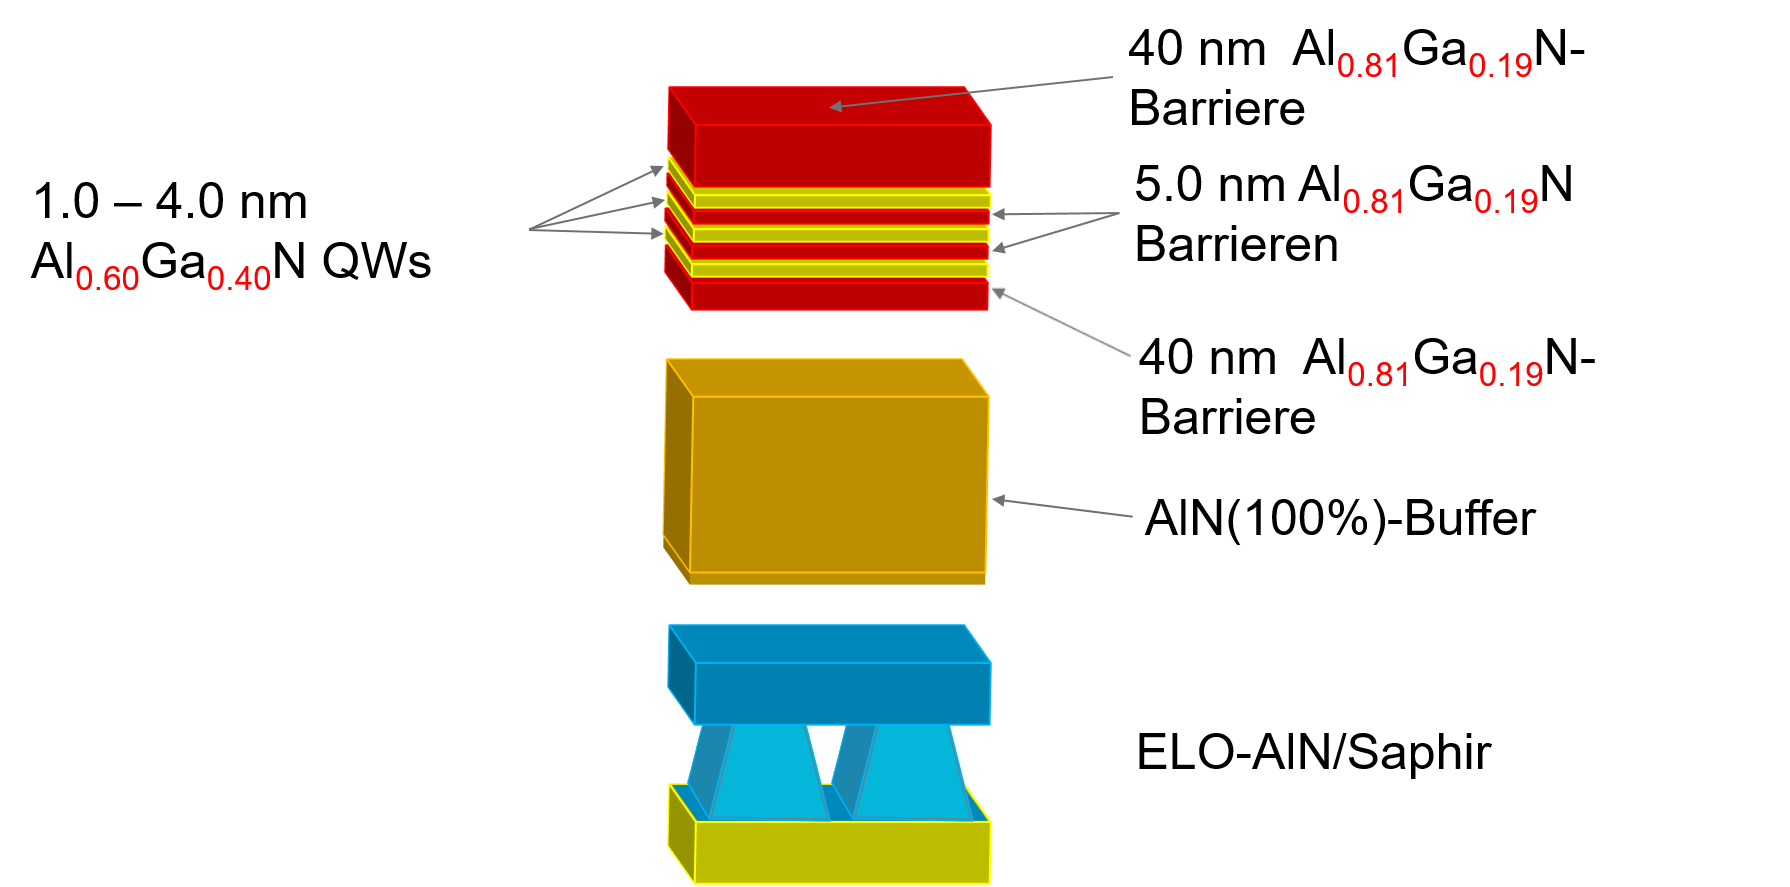
\includegraphics[width=\textwidth]{Bilder/MQWdickenSerie/undotiert}
		\caption{Aufbau der untersuchten MQW-Proben ohne dotierte Barrieren.}
    \label{fig:undotiert}
  \end{minipage}
	\hfill
  \begin{minipage}[t]{0.49\textwidth}
    \centering
    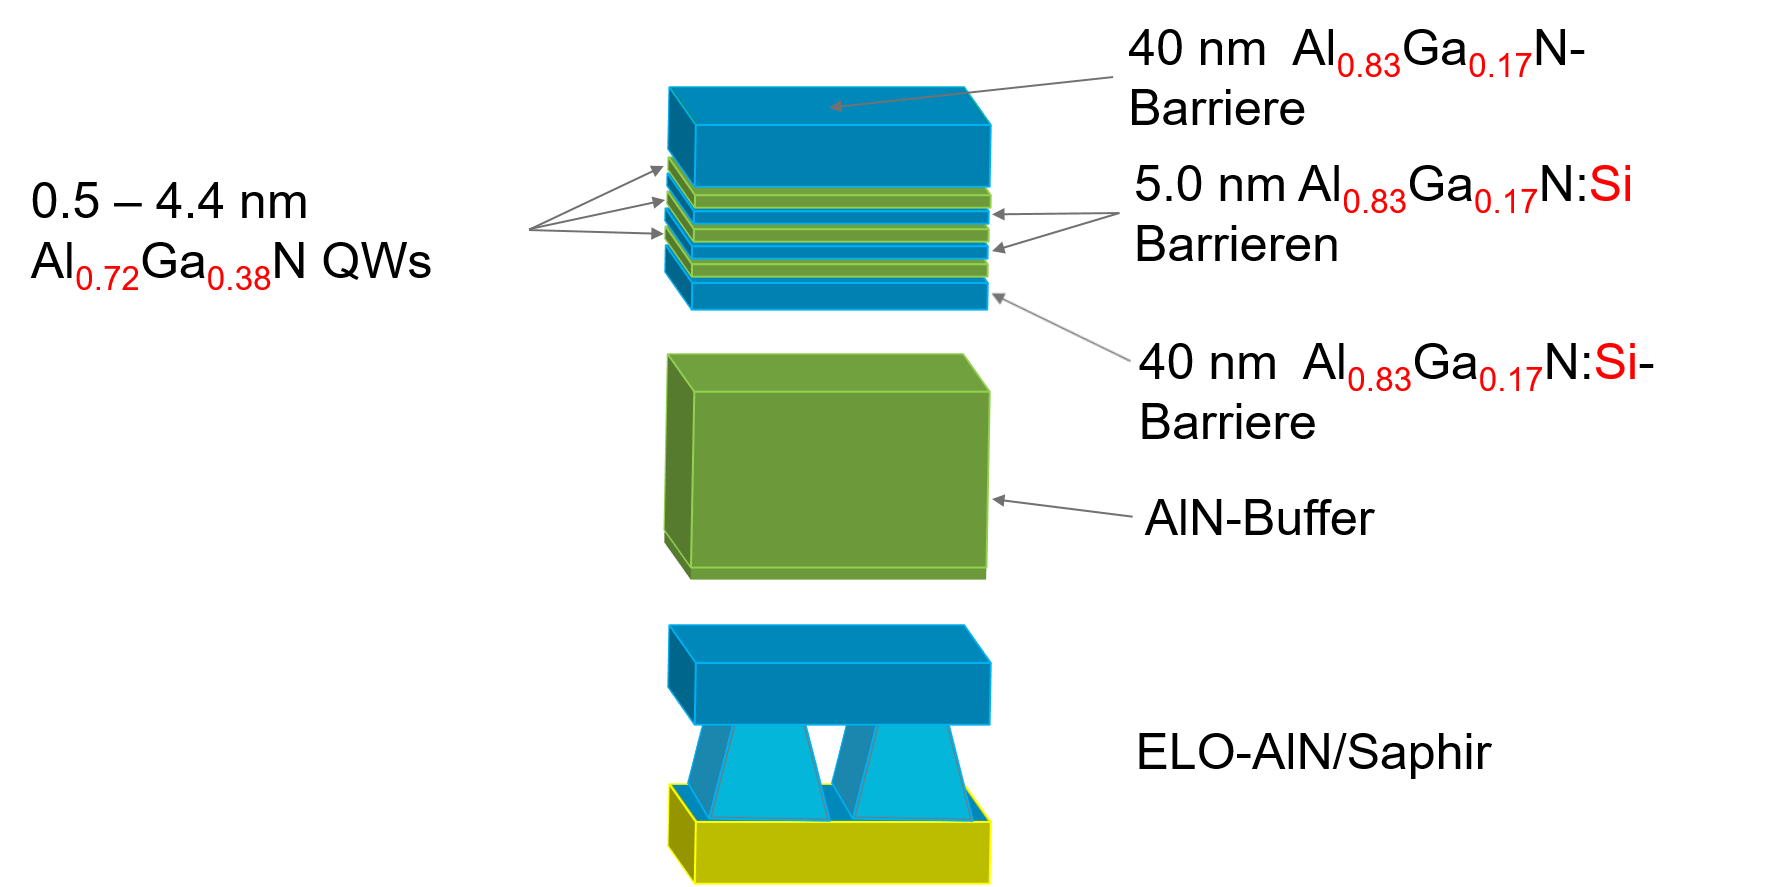
\includegraphics[width=\linewidth]{Bilder/MQWdickenSerie/dotiert}
		\caption{Aufbau der untersuchten MQW-Proben mit dotierten Barrieren.}
    \label{fig:dotiert}
  \end{minipage}
\end{figure}
\noindent 
Der Aufbau der Proben ohne dotierte Barrieren ist in Abbildung \ref{fig:undotiert} dargestellt.
Die aktive Zone setzt sich aus einem dreifach $ Al_{0.60}Ga_{0.40}N$-QW mit variierender Dicke $d$ ($d=1.0, 2.0, 3.0, 4.0 \thinspace nm$) und zwei $5 \thinspace nm$ dicken $ Al_{0.81}Ga_{0.19}N$-Barrieren zusammen. Diese liegen zwischen zwei $40 \thinspace nm$ dicken $ Al_{0.81}Ga_{0.19}N$-Barrieren von der eine die oberste Schicht darstellt. Darunter folgt eine AlN ($100\%$)-Bufferschicht, die auf einem ELO-AlN/Saphir Substrat aufgewachsen wurde. 
\newline
Abbildung \ref{fig:dotiert} zeigt den Aufbau der Proben mit dotierten Barrieren. Die aktive Zone setzt sich, aus zwei $5 \thinspace nm$ dicken und Si-dotierten $ Al_{0.83}Ga_{0.17}N:Si$-Barrieren zwischen denen sich drei $ Al_{0.72}Ga_{0.36}N$ QWs mit variierender Dicke $d$ ($d=0.5, 1.0, 2.2, 4.0 \thinspace nm$) befinden, zusammen. Diese liegen sich zwischen zwei $40 \thinspace nm$ dicken und Si-dotierten $ Al_{0.81}Ga_{0.19}N:Si$-Barrieren von der eine die oberste Schicht bildet. Darunter folgt eine AlN ($100\%$)-Bufferschicht die auf einem ELO-AlN/Saphir Substrat aufgewachsen wurde. 
\section{Ergebnisse}
Für die experimentelle Untersuchung wurden Photolumineszenzmessungen bei Tieftemperatur durchgeführt. Die aufgenommenen Spektren sind in den Abbildungen \ref{fig:undotiertSpektrumn} und \ref{fig:dotiertSpektrumn} dargestellt.
Es ist deutlich zu erkennen, dass mit sinkender QW-Dicke $d$ die Emissionsenergie steigt.
\begin{figure}[H]
  \centering
  \begin{minipage}[t]{0.45\textwidth}
    \centering
    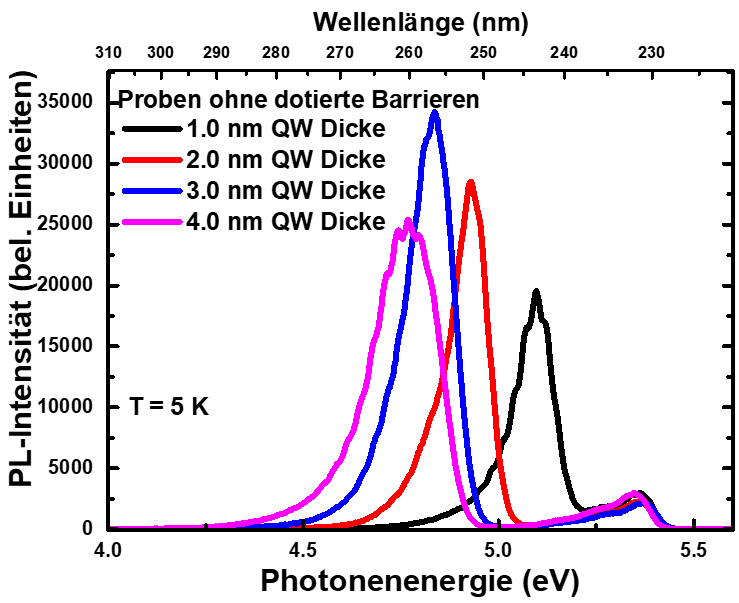
\includegraphics[width=\textwidth]{Bilder/MQWdickenSerie/spektrumUndotiert}
		\caption{PL-Spektren der untersuchten MQW-Proben ohne dotierte Barrieren.}
    \label{fig:undotiertSpektrumn}
  \end{minipage}
	\hfill
  \begin{minipage}[t]{0.45\textwidth}
    \centering
    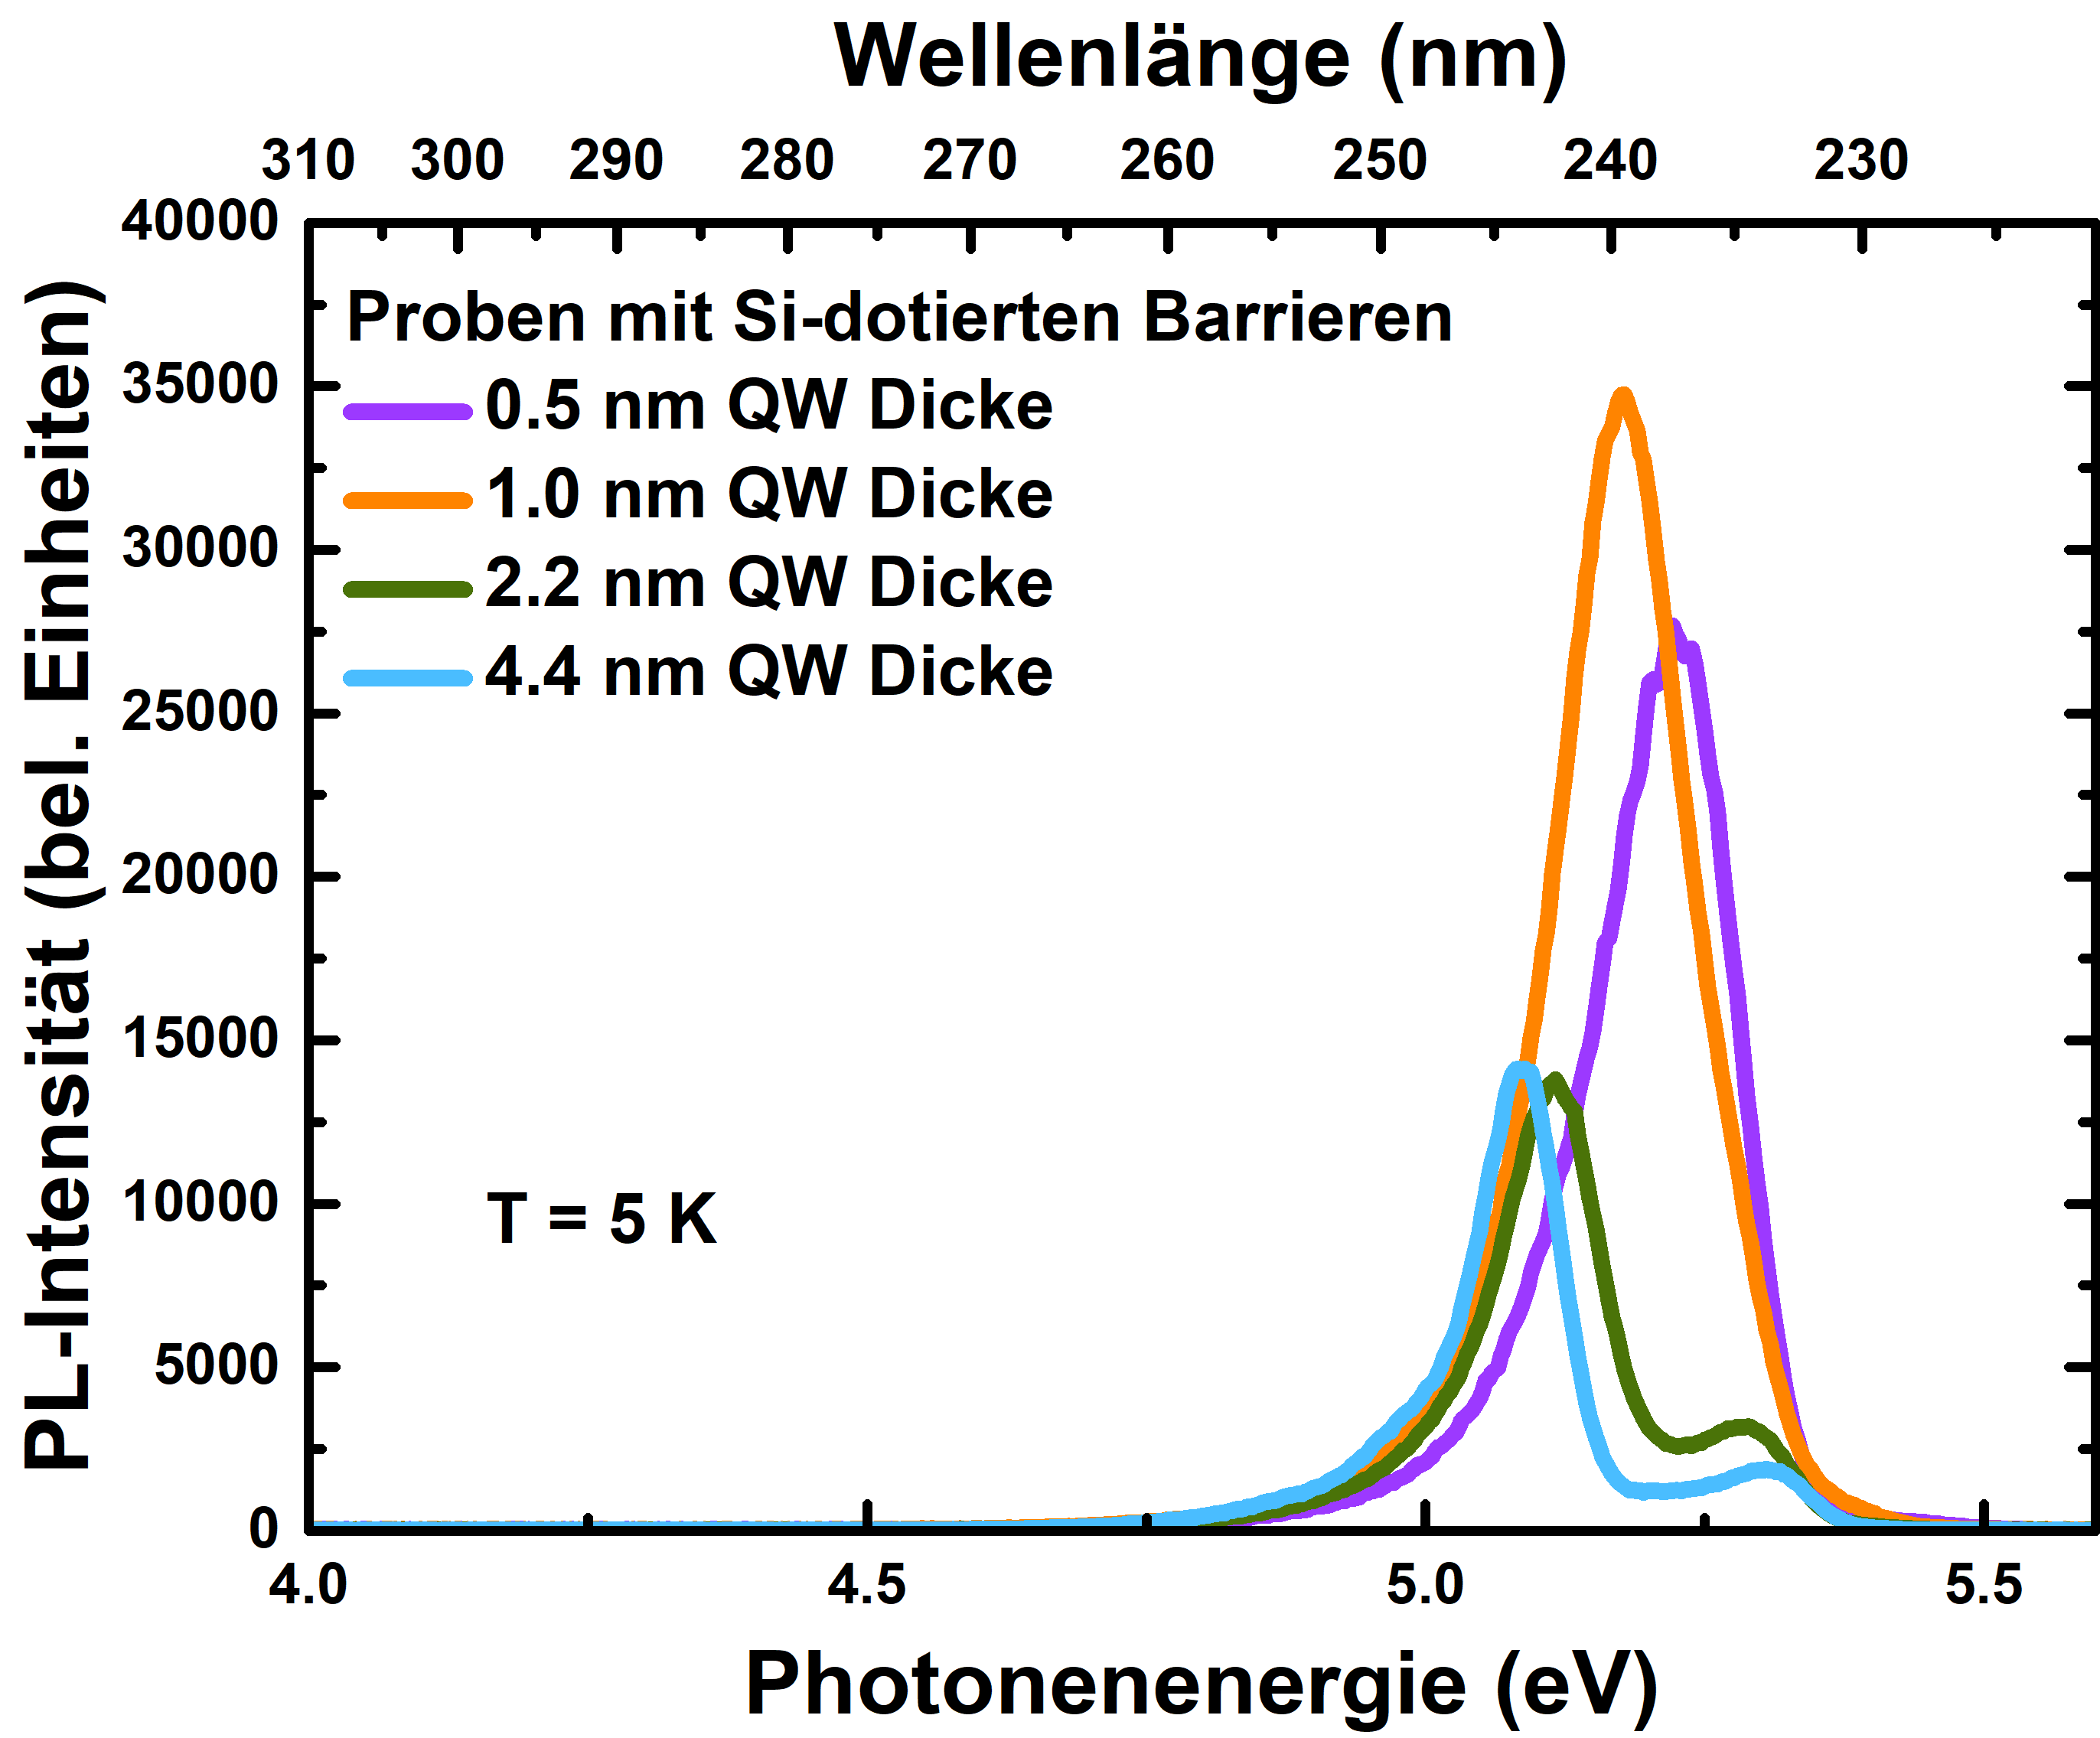
\includegraphics[width=\linewidth]{Bilder/MQWdickenSerie/spektrumDotiert}
		\caption{PL-Spektren der untersuchten MQW-Proben mit dotierten Barrieren.}
    \label{fig:dotiertSpektrumn}
  \end{minipage}
\end{figure}
\noindent 
Die Gründe hierfür sind die Übergangsenergien, die mit steigender QW-Dicke \cite{doi:10.1063/1.371241} sinken. 
Die Emissionsenergien beider Serien unterscheiden sich, da die aktiven Zonen unterschiedliche Zusammensetzungen in den Barrieren und QWs (siehe Abb. \ref{fig:undotiert} und \ref{fig:dotiert}) aufweisen. 
\newline
In den Abbildungen \ref{fig:undotiertint} und \ref{fig:dotiertint} ist die integrierte Intensität gegen die Anregungsleistungsdichte bei Tieftemperatur für die Proben mit dotierter und undotierter Barriere in doppeltlogarithmischer Darstellung aufgetragen.
\begin{figure}[H]
  \centering
  \begin{minipage}[t]{0.49\textwidth}
    \centering
    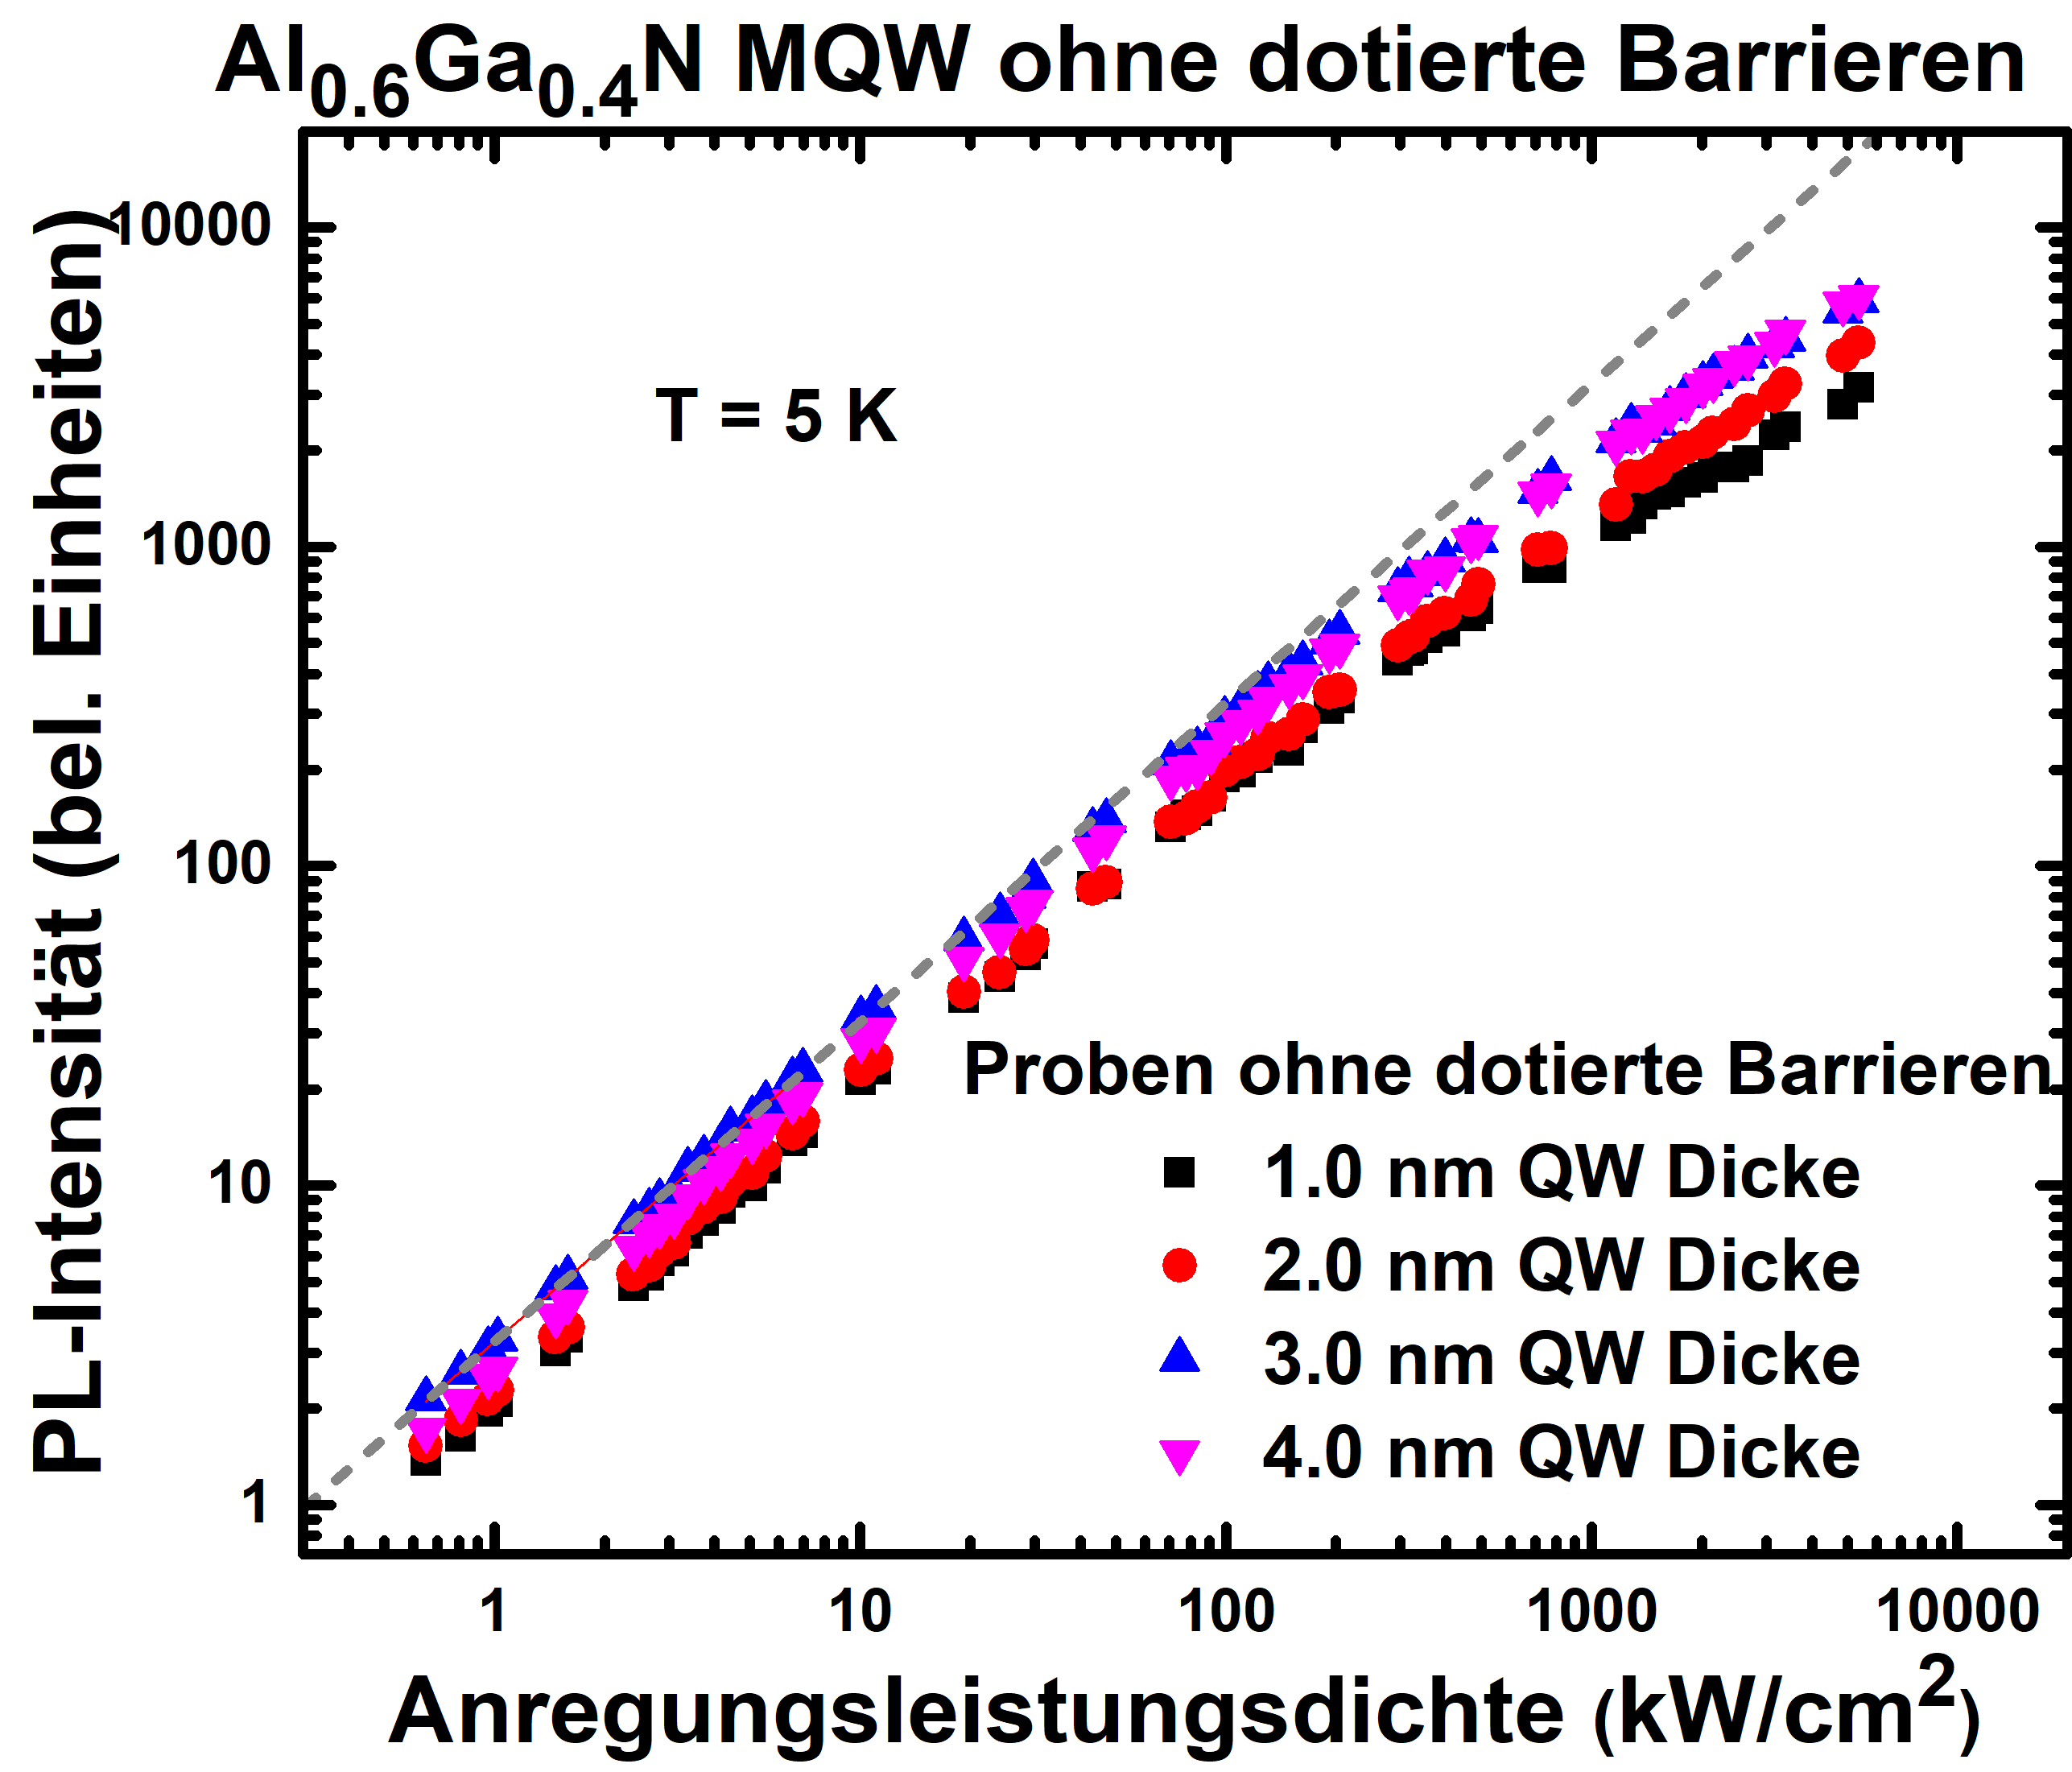
\includegraphics[width=\textwidth]{Bilder/MQWdickenSerie/intTTundotiert.png}
		\caption{Integrierte Intensität in doppeltlogarithmischer Darstellung in Abhängigkeit der Anregungsleistungsdichte bei Tieftemperatur für die Proben mit undotierter Barriere.}
    \label{fig:undotiertint}
  \end{minipage}
	\hfill
  \begin{minipage}[t]{0.49\textwidth}
    \centering
    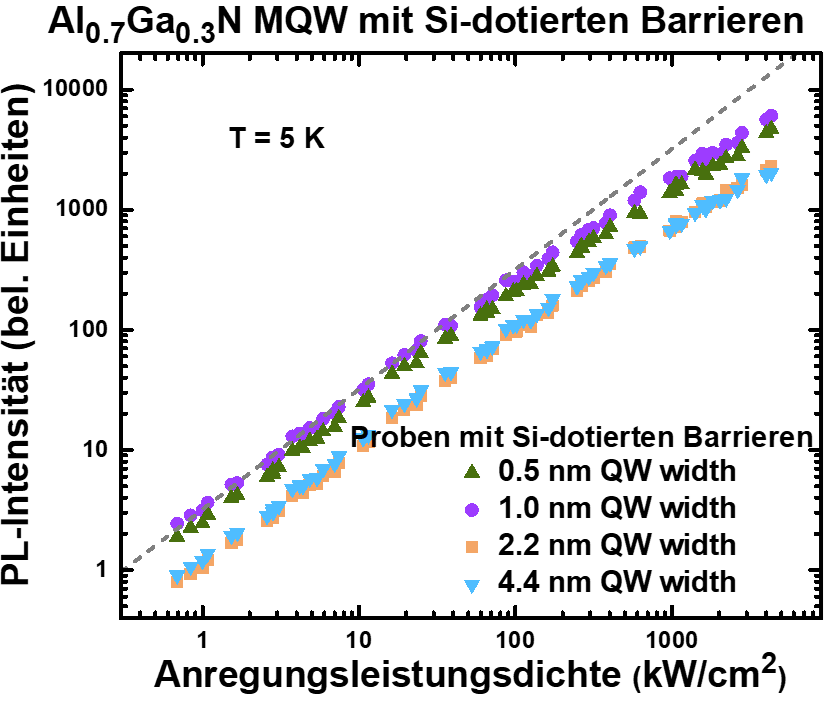
\includegraphics[width=\linewidth]{Bilder/MQWdickenSerie/intTTdotierte.png}
		\caption{Integrierte Intensität in doppeltlogarithmischer Darstellung in Abhängigkeit der Anregungsleistungsdichte bei Tieftemperatur für die Proben mit dotierter Barriere.}
    \label{fig:dotiertint}
  \end{minipage}
\end{figure}
\noindent 
Im Bereich geringer Anregungsleistungsdichten zeigt sich für beide Serien eine lineare Steigung (gestrichelte Linie), die mit zunehmender Anregungsleistungsdichte in einen nichtlinearen Verlauf übergeht. Dieser ist wie in Kapitel \ref{chap:auger} beschrieben, vermutlich auf die Auger-Rekombination zurückzuführen.
Die integrierten Intensitäten befinden sich für die Proben mit undotierter Barriere bei Tieftemperatur für alle QW-Dicken auf einem vergleichbaren Niveau.
\newline
Die Proben mit einer QW-Dicke von $3.0 \thinspace nm$ und $4.0 \thinspace nm$ emittieren am hellsten und die Proben mit $2.0 \thinspace nm$ und $1.0 \thinspace nm$ QW-Dicke etwas schwächer. 
Zwar heben sich die Verläufe für die verschiedenen Proben voneinander ab, so sind diese Unterschiede jedoch marginal und im Rahmen der Streuung, die durch die Justage und Positionen im PL-Aufbau zu erwarten sind. Gleiches gilt für die Proben mit dotierter Barriere wie Abbildung \ref{fig:dotiertint} zeigt. 
Dort fallen die Proben mit QW-Dicken von $2.2 \thinspace nm$ und $4.4 \thinspace nm$ im Vergleich zu den anderen Dicken deutlicher ab. Diese Unterschiede bleiben jedoch immer noch im Rahmen der Streuung.  
\begin{figure}[H]
  \centering
  \begin{minipage}[t]{0.49\textwidth}
    \centering
    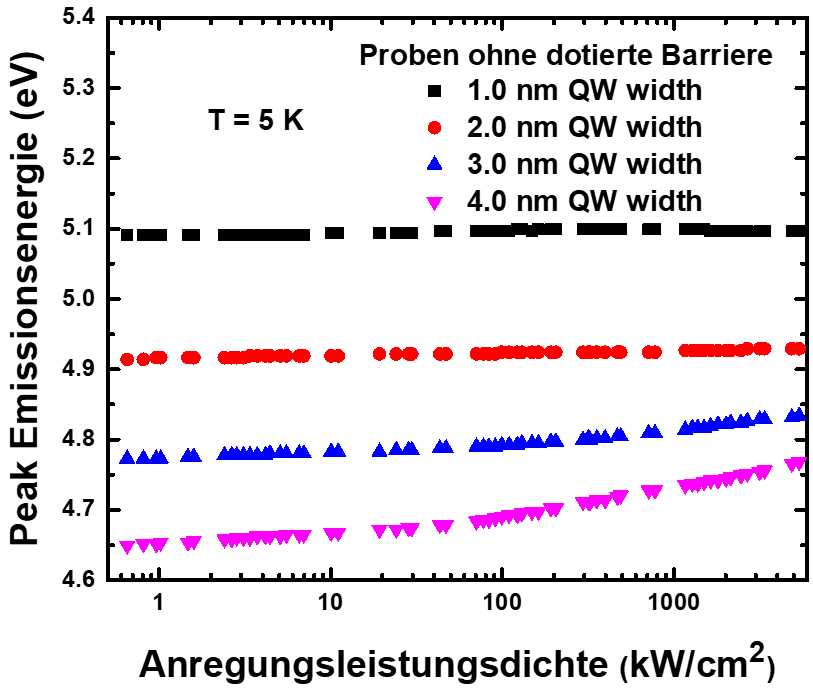
\includegraphics[width=\textwidth]{Bilder/MQWdickenSerie/PeakEnergieUndotiert.png}
		\caption{Peak-Emissionsenergie in Abhängigkeit der Anregungsleistungsdichte bei Tieftemperatur der untersuchten MQW-Proben ohne dotierte Barrieren.}
    \label{fig:undotiertpeak}
  \end{minipage}
	\hfill
  \begin{minipage}[t]{0.49\textwidth}
    \centering
    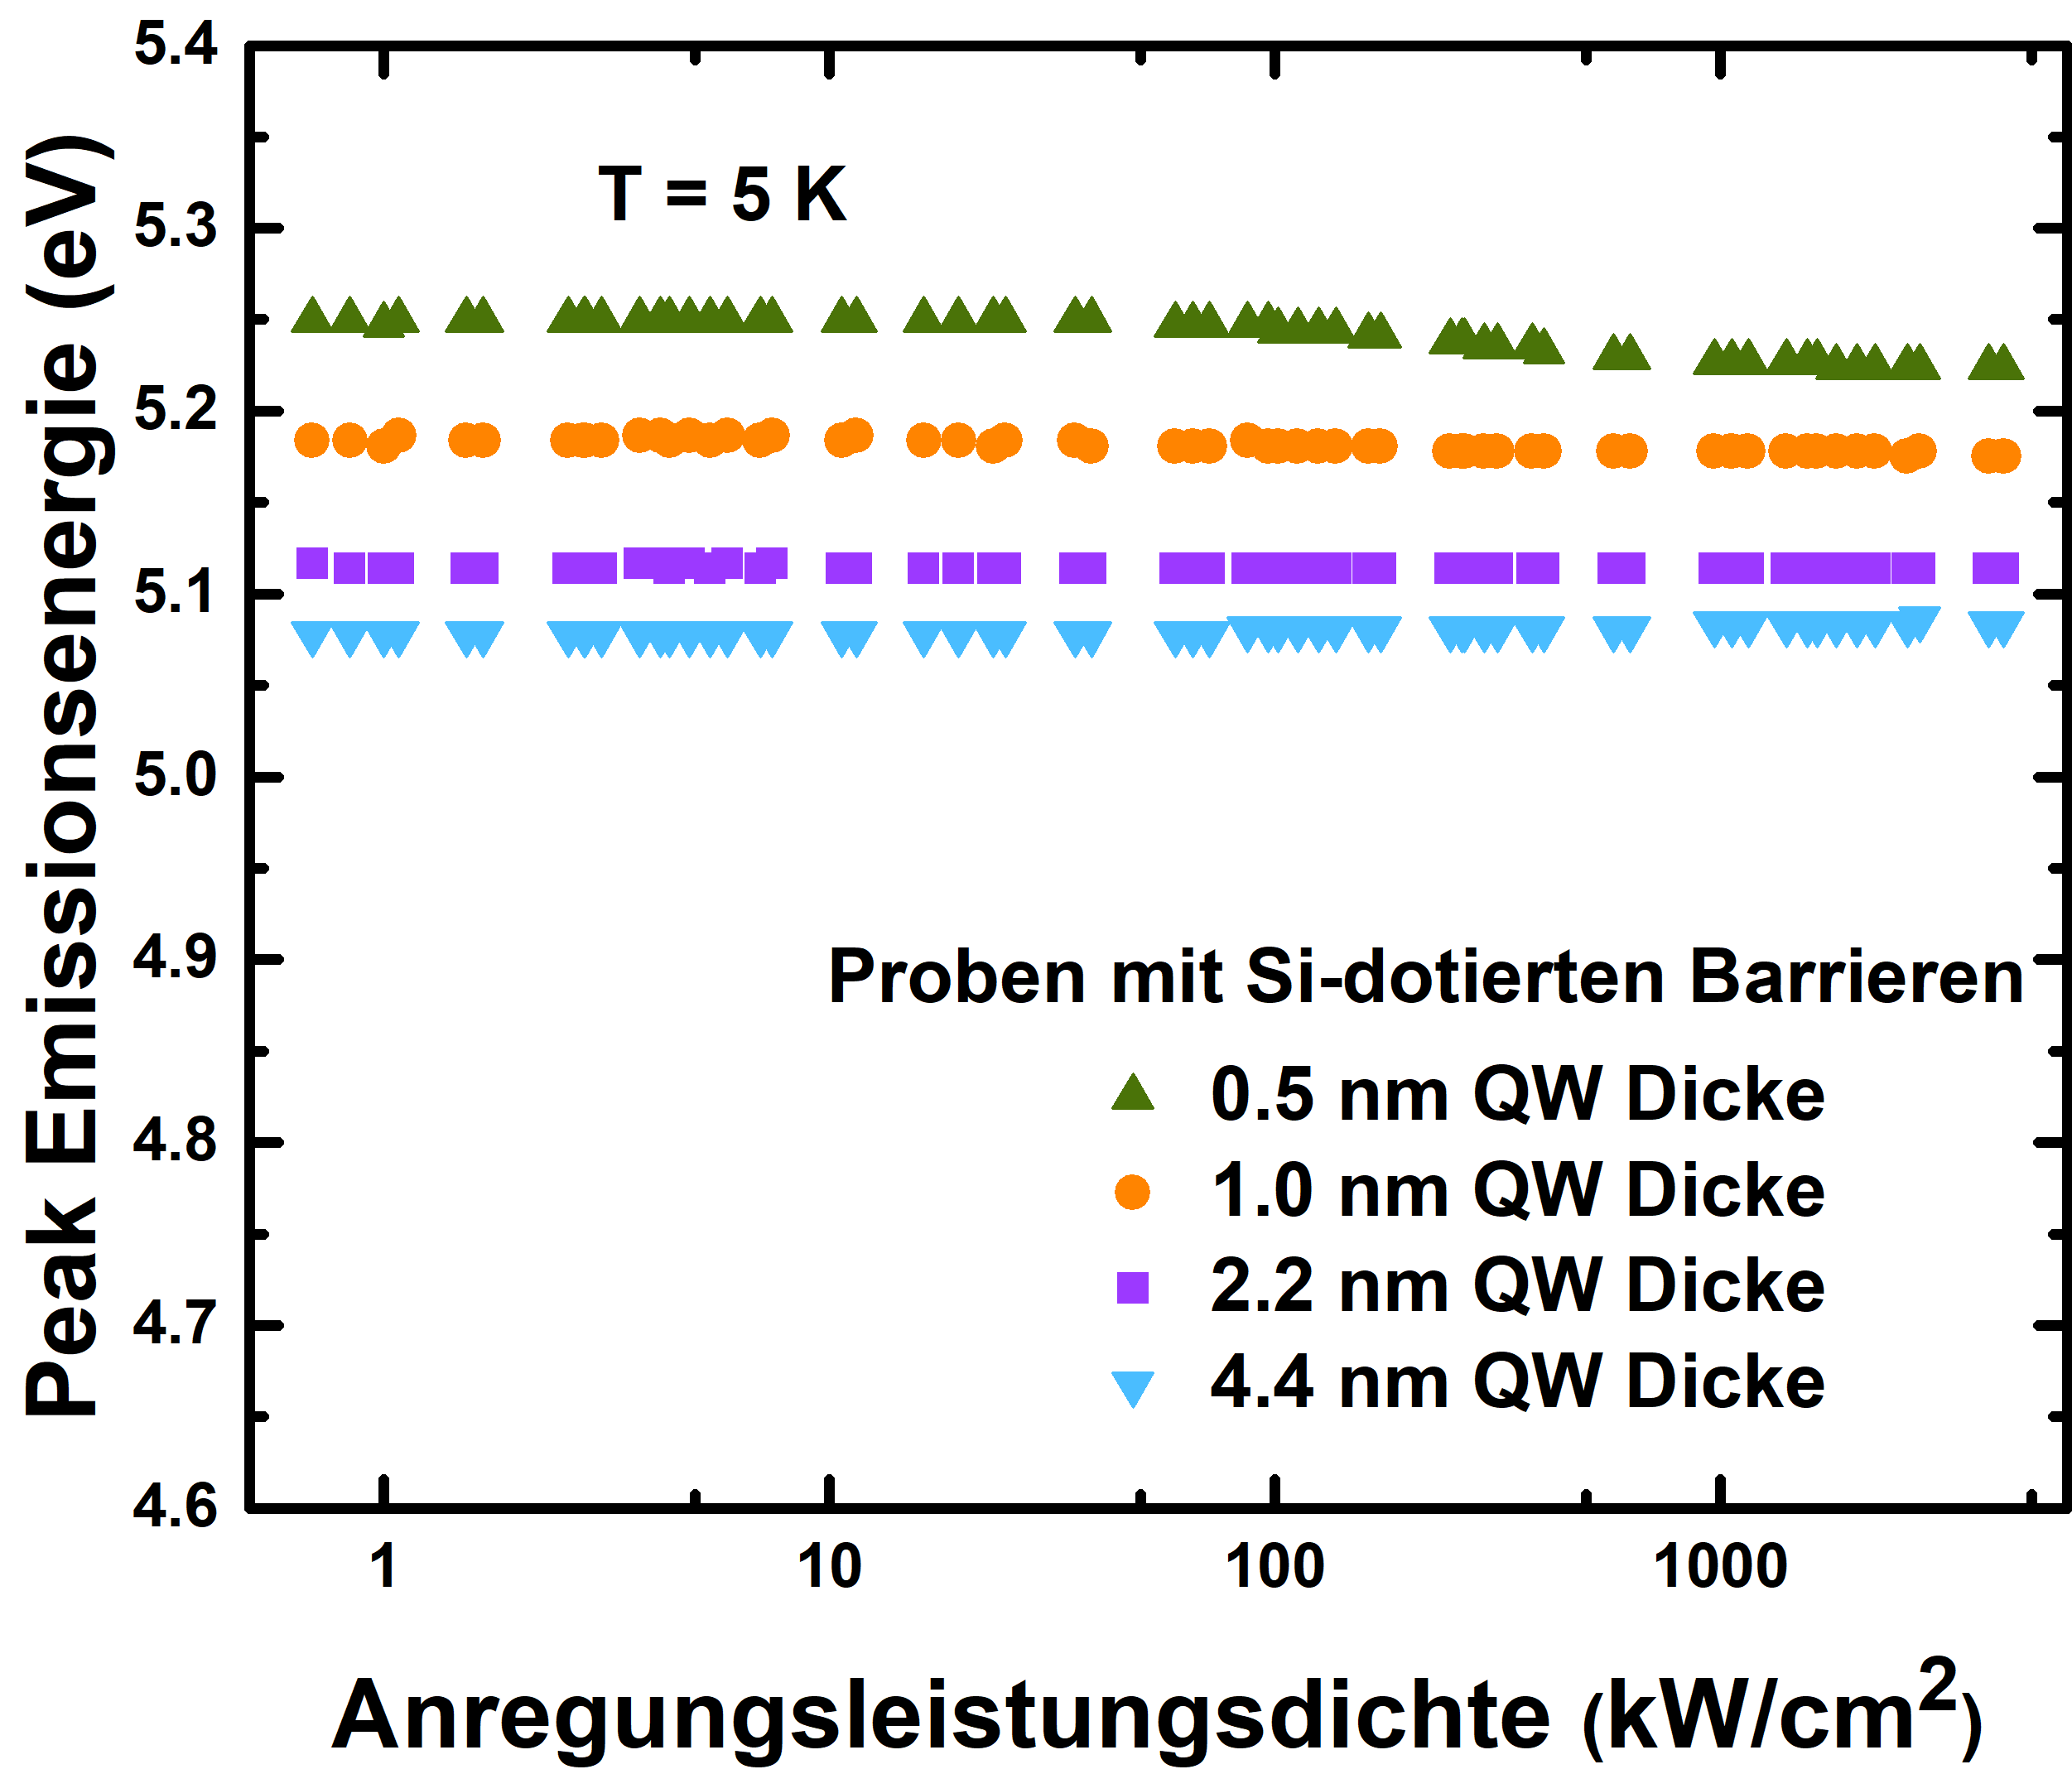
\includegraphics[width=\linewidth]{Bilder/MQWdickenSerie/PeakEnergieDotiert.png}
		\caption{Peak-Emissionsenergie in Abhängigkeit der Anregungsleistungsdichte bei Tieftemperatur der untersuchten MQW-Proben mit dotierten Barrieren.}
    \label{fig:dotiertpeak}
  \end{minipage}
\end{figure}
\noindent 
Die Abbildungen \ref{fig:undotiertpeak} und \ref{fig:dotiertpeak} zeigen die Peak-Emissionsenergie aufgetragen gegen die Anregungsleistungsdichte bei Tieftemperatur. 
Für die Proben mit undotierten Barrieren ist in Abbildung \ref{fig:undotiertpeak} zu erkennen, dass mit steigender Anregungsleistungsdichte die Peak-Emissionsenergie steigt. Der Grund hierfür ist das Screening des QCSE \cite{doi:10.1063/1.1763211}. Dieser Screening-Effekt wird größer mit kleiner werdender QW-Dicke, weil bei kleinerer QW-Dicke die Auswirkung des QCSE geringer ausfällt. Dies bedeutet, dass eine geringere Ladungsträgerdichte im QW notwendig ist, um die Bandverbiegung und damit die Separation der Elektron- und Lochwellenfunktion aufzuheben. 
\newline
Damit einhergehend ist die Verschiebung der Peak-Emissionsenergien bei der Probe mit einer QW-Dicke von $4.0 \thinspace nm$ von $4.65 \thinspace eV$ bei der geringsten Anregungsleistungsdichte zu $4.77 \thinspace eV$ bei der höchsten Anregungsleistungsdichte am stärksten. 
\newline 
Die Probe mit einer QW-Dicke von $1.0 \thinspace nm$ zeigt dagegen keine Verschiebung der Peak-Emissionsenergien. Dies bestätigt, dass für kleine Dicken $d$ eine geringere Ladungsträgerdichte für das Screening des QCSE notwendig wird.
\newline
Die Proben mit dotierten Barrieren zeigen ein ähnliches Verhalten, wie in Abbildung \ref{fig:dotiertpeak} dargestellt ist. So sind die Peak-Emissionsenergien für die Proben mit einer QW-Dicke von 
$1.0 \thinspace nm$, $2.2 \thinspace nm$ und $4.4 \thinspace nm$ nahezu konstant über den ganzen Bereich der Anregungsleistungsdichte.
Der Grund hierfür könnte sein, dass bereits eine höhere Anzahl an Ladungsträgern durch die Dotierung zur Verfügung stehen, die zusätzlich zur externen Anregung dazu beitragen, den Effekt des QCSE zu reduzieren.
\newline
Auffällig ist, dass sich die Emissionsenergie der Probe mit der geringsten QW-Dicke von $0.5 \thinspace nm$ mit steigender Anregungsleistungsdichte hin zu kleineren Energien verschiebt. Die Gründe für dieses Verhalten sind bisher unklar.
\begin{figure}[H]
  \centering
  \begin{minipage}[t]{0.49\textwidth}
    \centering
    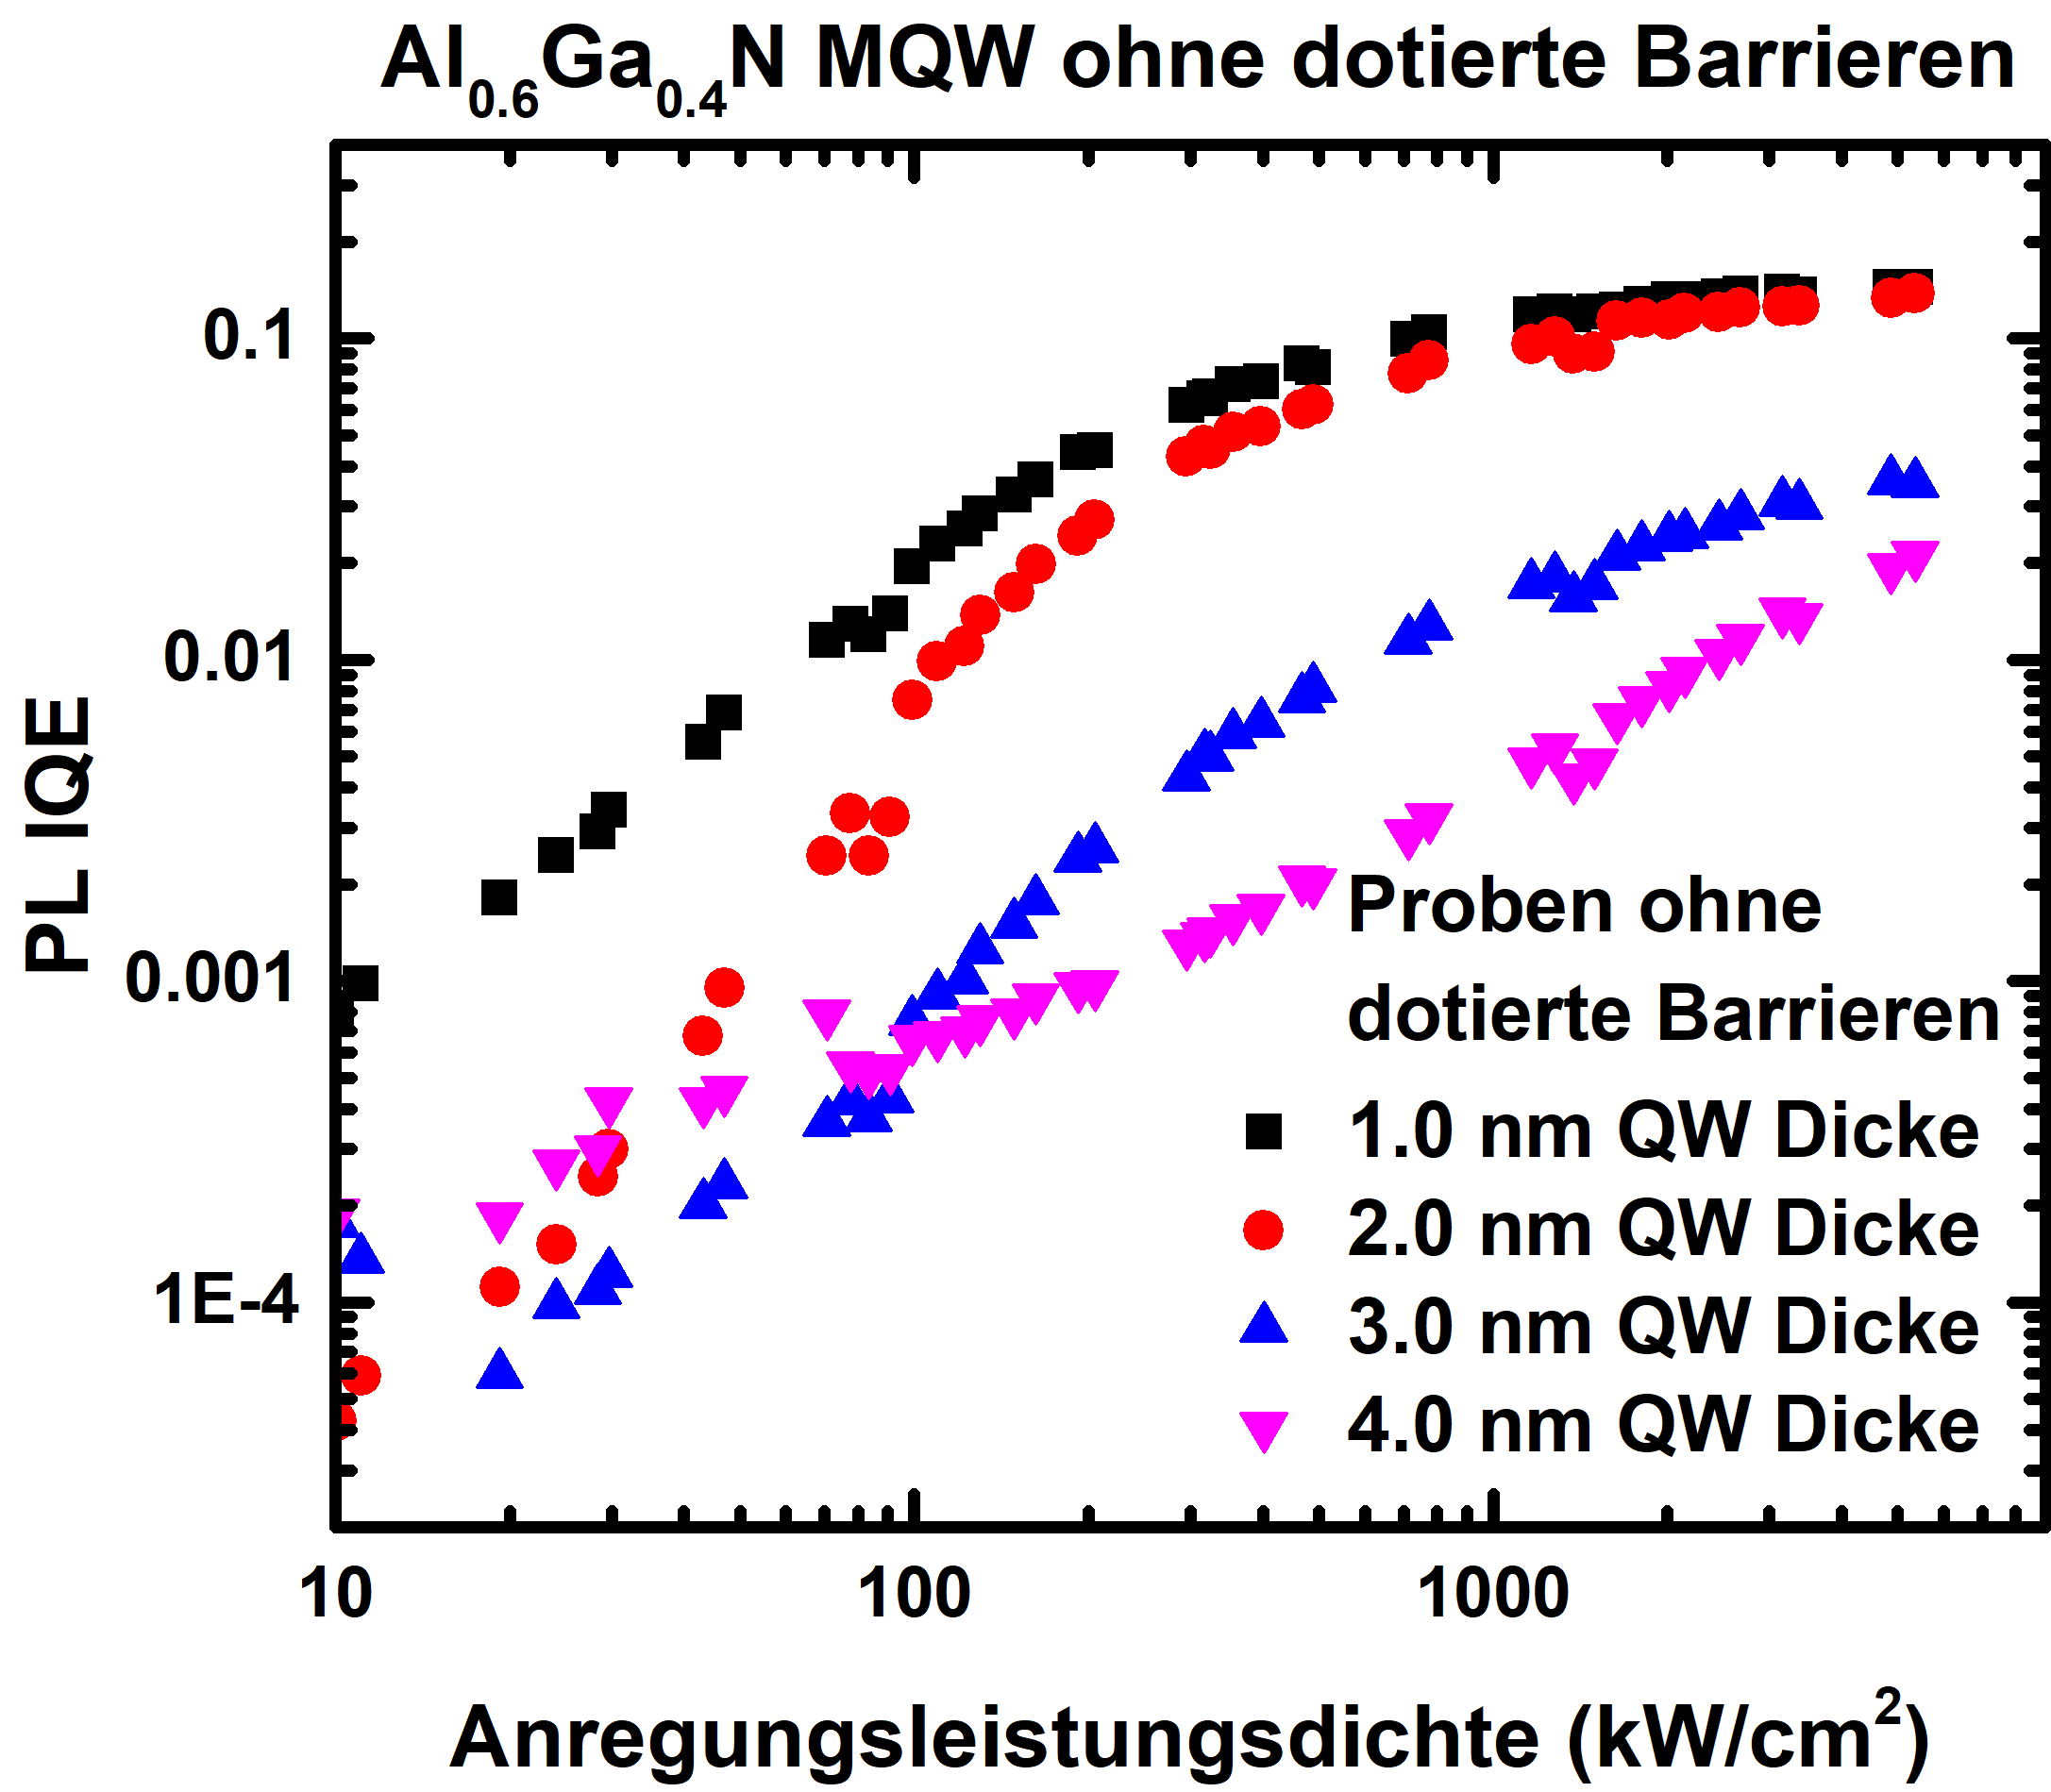
\includegraphics[width=\textwidth]{Bilder/MQWdickenSerie/IQEundotiert.png}
		\caption{IQE in Abhängigkeit der Anregungsleistungsdichte bei Raumtemperatur der untersuchten MQW-Proben ohne dotierte Barrieren.}
    \label{fig:undotiertIQE}
  \end{minipage}
	\hfill
  \begin{minipage}[t]{0.49\textwidth}
    \centering
    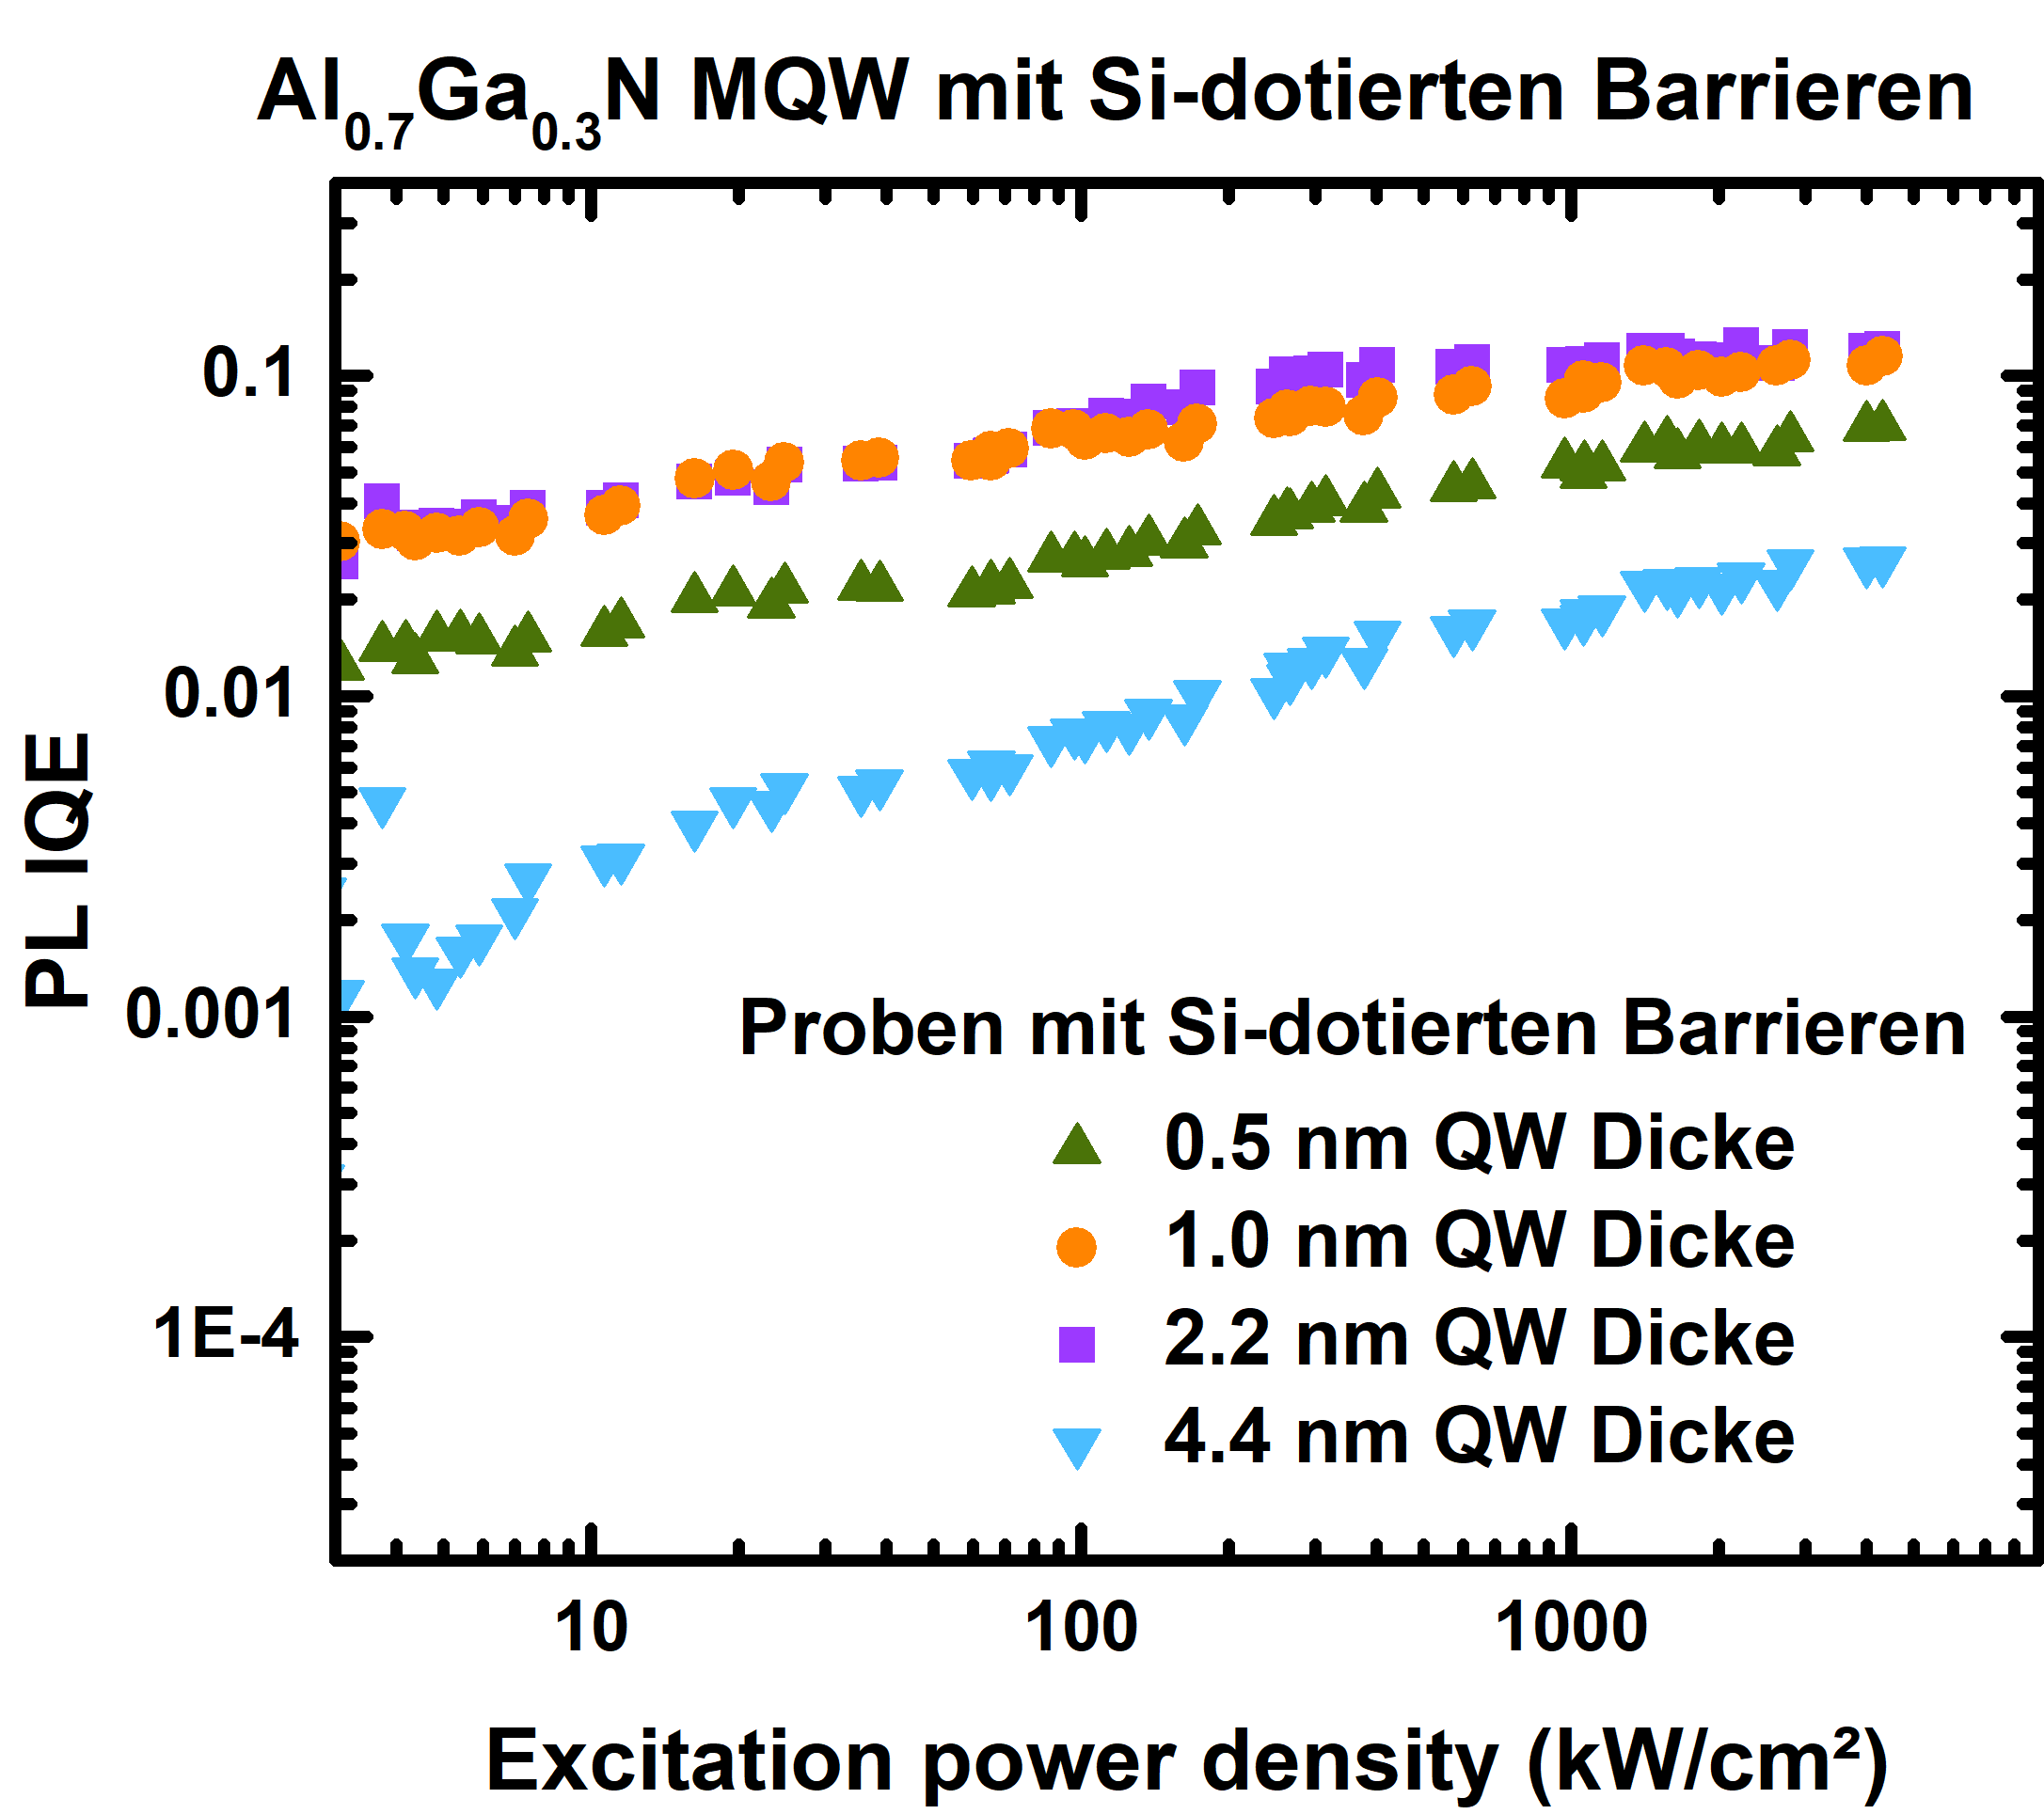
\includegraphics[width=\linewidth]{Bilder/MQWdickenSerie/IQEdotiert.png}
		\caption{IQE in Abhängigkeit der Anregungsleistungsdichte bei Raumtemperatur der untersuchten MQW-Proben.}
    \label{fig:dotiertIQE}
  \end{minipage}
\end{figure}
\noindent 
Die Ergebnisse der IQE bei Raumtemperatur für die Proben ohne und mit dotierten Barrieren sind in den Abbildungen 
\ref{fig:undotiertIQE} und \ref{fig:dotiertIQE} zu sehen. Für beide Probenserien zeigt sich, dass aufgrund des QCSE die IQE für breite QWs 
($3.0 - 4.4 \thinspace nm$) geringer ausfällt. Ebenso verhält es sich bei besonders geringen Dicken ($0.5\thinspace nm$), bedingt durch den schlechteren Ladungsträgereinschluss. Die höchsten IQE werden für QW-Dicken von $1.0 \thinspace nm- 2.2 \thinspace nm$ gemessen. Die Proben ohne Dotierung mit QW-Dicken von $1.0 \thinspace nm$ und $2.0\thinspace nm$ haben beide eine IQE von ca. $0.145$ bei höchster Anregungsleistungsdichte.
\newline
Die Proben mit dotierten Barrieren und QW-Dicken von $1.0 \thinspace nm$ und $2.2\thinspace nm$ haben beide eine IQE von ca. $0.121$ bei höchster Anregungsleistungsdichte. 
\newline
Anhand der Ergebnisse für die Proben mit dotierten Barrieren ist zu erkennen, dass die Si-dotierung einen deutlichen Einfluss auf den Verlauf der IQE hat. So ist die Ordinate der IQEs für diese Proben deutlich höher, wie Abbildung \ref{fig:dotiertIQE} zeigt. Die Dotierung führt sichtbar zu höheren IQEs bei geringen Anregungsleistungsdichten. Die Steigung mit wachsender Anregungsleistungsdichte ist jedoch im Vergleich geringer, sodass die höchsten IQEs für beide Serien ungefähr den selben Wert zwischen $0.121$ und $0.145$ im Bereich hoher Anregungsleistungsdichten einnehmen. 
\newline
Der Grund für dieses unterschiedliche Verhalten ist durch den Effekt der Dotierung auf den QCSE zu erklären. Durch die Si-Dotierung werden Ladungsträger in die Struktur gebracht, die neben der durch Anregung extern zugeführten Ladungsträgerdichte zu einer zusätzlichen Abschirmung der Polarisationsfelder führen. Dieser Effekt ist am deutlichsten bei geringen Anregungsleistungsdichten zu sehen und verliert an Einfluss im Bereich großer Anregungsleistungsdichten, da die durch Anregung generierte Ladungsträgerdichte den Effekt des Screenings deutlich dominiert.

\iffalse
\section{Einfluss der Siliziumdotierung auf die IQE}

Um die Unterschiede in der IQE für dotierte- und undotierte Barrieren zu klären, soll nun das ABC-Modell erweitert werden, um den Effekt der Dotierung mit einzubeziehen. 
Das ABC-Modell stellt nur eine Vereinfachung dar und berücksichtigt nicht alle vorkommenden Effekte wie beispielsweise Lokalisierung, Screening durch Ladungsträger und Dotierung. 
Der Effekt der Dotierung spielt dabei eine besonders wichtige Rolle, da eine Si-Dotierung für das erreichen einer hohen Leitfähigkeit üblich in UV-LEDs ist \cite{doi:10.1063/1.1492316}.
Nach \cite{schub} soll mit Hilfe der Ratengleichungen gezeigt werden, dass sich mit der Annahme einer Dotierung,
der Anteil der strahlenden Rekombination ändert.
\newline
\begin{figure}[H]
    \centering
    \begin{minipage}[t]{0.49\linewidth}
        \centering
        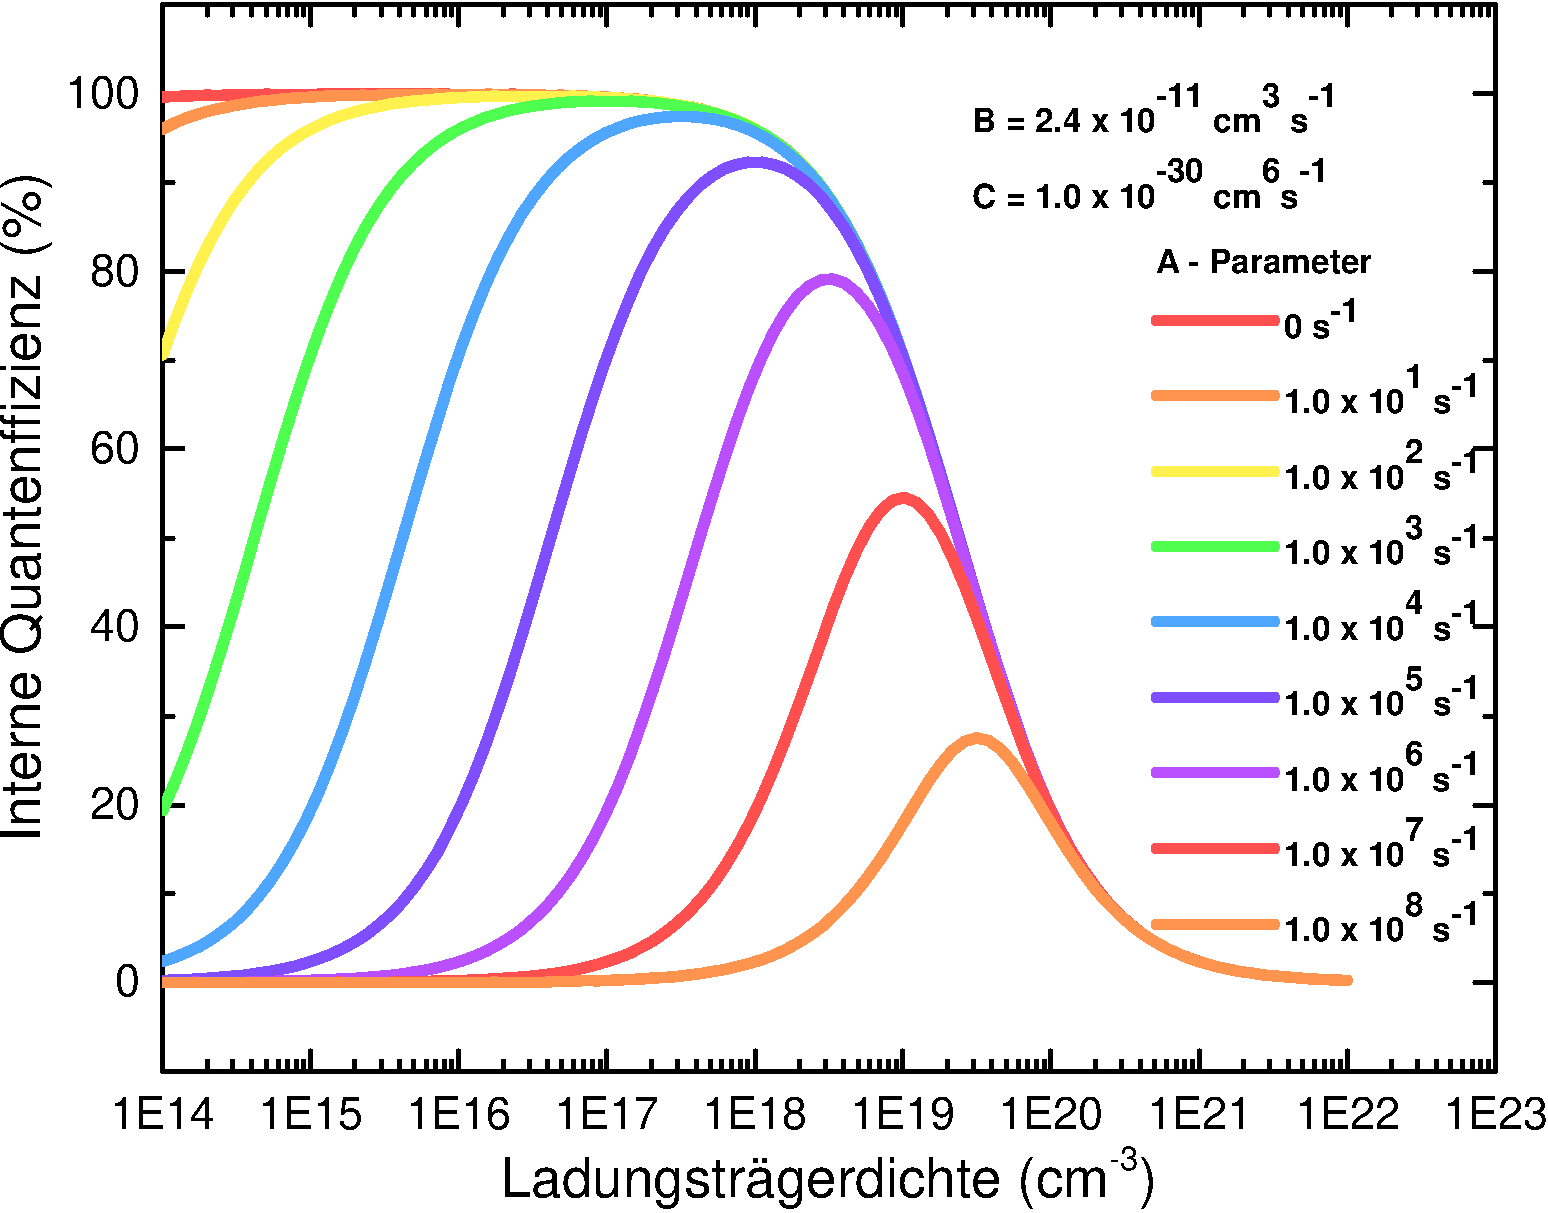
\includegraphics[width=\linewidth]{Bilder/IQEohneDotierungVerschAParams.pdf}
        \caption{Die Grafik zeigt}
        \label{fig:iqenorm}
    \end{minipage}% <- sonst wird hier ein Leerzeichen eingefügt
    \hfill
    \begin{minipage}[t]{0.49\linewidth}
        \centering
        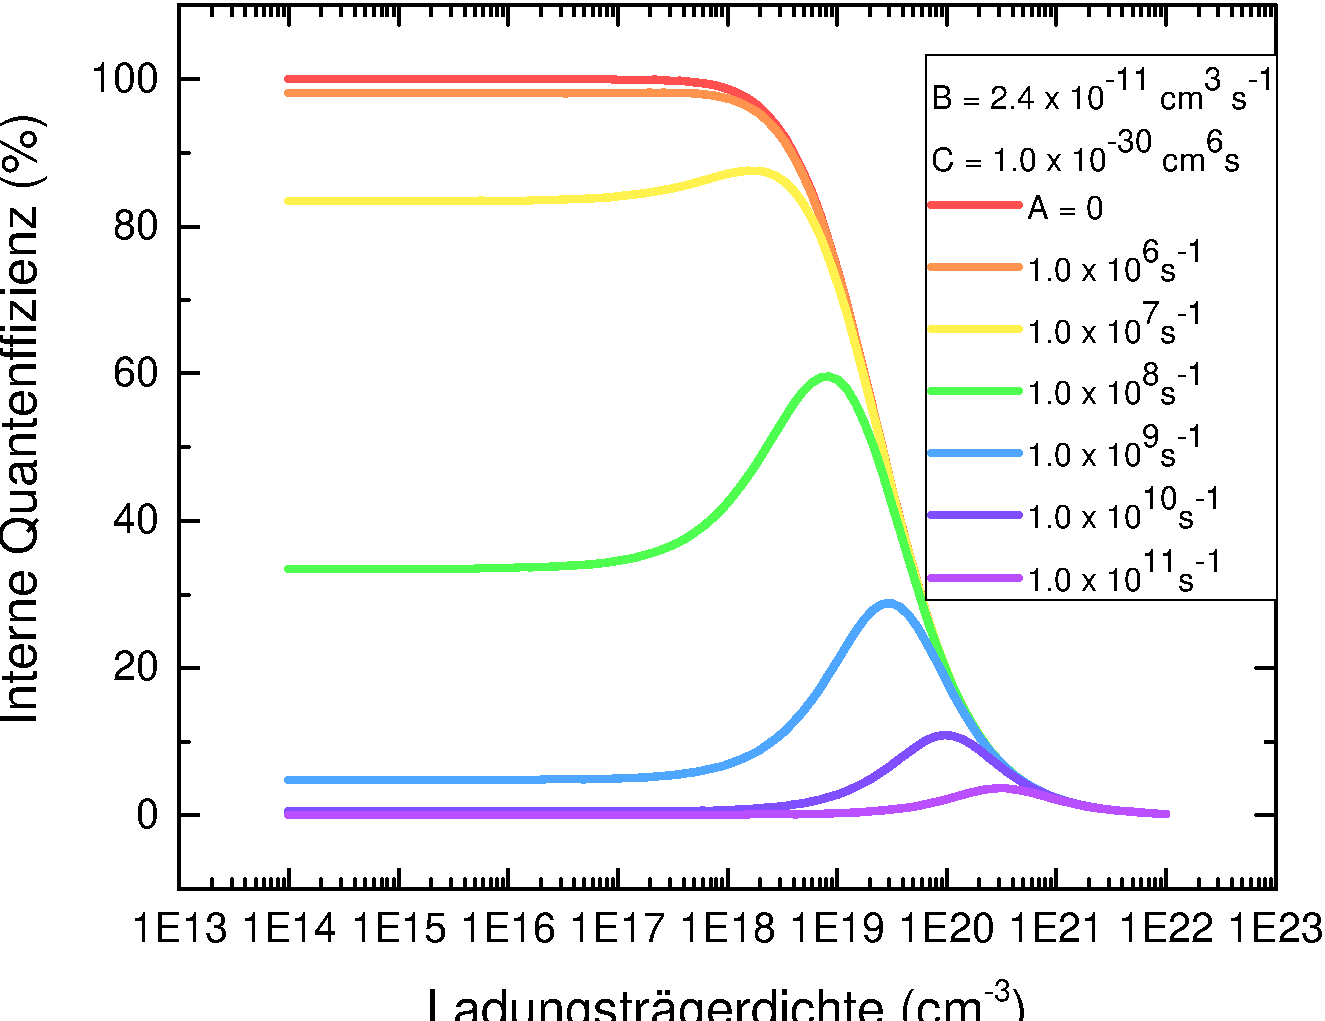
\includegraphics[width=\linewidth]{Bilder/IQEmitDotierungVerschAParams.pdf}
        \caption{Die Grafik zeigt  }
        \label{fig:iqedot}
    \end{minipage}
\end{figure}
\vspace{0.1cm}
\noindent
Jeder dotierte oder undotierte Halbleiter hat zwei Arten von Ladungsträgern, Elektronen und Löcher.
Im Gleichgewicht, bedeutet ohne externe Anregung durch Absorption von Licht oder Injektion von Elektronen, ist das Produkt von Elektronen- und Lochkonzentration eine konstante Größe.
\begin{equation}
    n_0 \cdot p_0 = n_i^2
    \label{eq:constant}
\end{equation}
Hierbei sind $n_0$ und $p_0$ die Elektron- und Lochkonzentration unter Gleichgewichtsbedingung und $n_{i}$ damit die intrinsische Ladungsträgerkonzentration.
Werden zusätzlich die durch Anregung erzeugten Ladungsträger betrachtet, so ist die Gesamtladungsträgerkonzentration gegeben als Summe der Anregungs- und Gleichgewichtsladungsträger. 
\begin{equation}
    n_{ges} = n_0 + n \medspace \text{und} \medspace  p_{ges} = p_0 +  n 
\end{equation}
Hierbei sind $ n$ und $p$ die Anregungsladungsträger. 
Die Anzahl der stattfindenden Rekombination zwischen Elektronen und Löchern sind direkt proportional zur Elektronen-und Ladungsträgerkonzentration, so gilt, $R \propto n \cdot p $. Mit einer Proportionalitätskonstante, wird die Rekombinationsrate pro Zeit und Volumen definiert als
\begin{equation}
    R = - \frac{dn_{ges}}{dt} = - \frac{dp_{ges}}{dt} = B \cdot n_{ges} \cdot p_{ges}
\end{equation}
Weil Elektronen und Löcher bei Anregung paarweise erzeugt werden und verschwinden (durch Rekombination), gilt
\begin{equation}
    \label{eq:gleich}
    n(t) =  p(t)
\end{equation}
Die radiative Rekombinationsrate wird dann mit $p_{0} = 0$ und Gleichung \ref{eq:gleich} zu
\begin{align}
\begin{split}
    R_{rad} &= B \cdot (n_0 + n)  \cdot (p_0 + p) ,
    \\
    R_{rad} &= B \cdot (n_0 + n) \cdot (n) ,
    \\
    R_{rad} &= B \cdot n^2 + B \cdot n \cdot n_0
\end{split}
\end{align}
Dabei beschreibt $n_{0}$ die Ladungsträgerkonzentration durch die Silizumdotierung. 
Somit wird die IQE zu:
\begin{equation}
    IQE = \frac{B \cdot n^2 + B \cdot n \cdot n_{0}}{A \cdot n + B \cdot n^2  + B \cdot n \cdot n_{0}+ C \cdot n^3} 
    \label{eq:dopediqe}
\end{equation}
Und hat einen enormen Einfluss auf die Ordinate, wie in Abb. \ref{fig:iqedot} zu sehen ist und zeigen damit im Vergleich mit der experimentell ermittelten IQE in Abbildung \ref{fig:dotiertIQE} für die Serie mit dotierten Barriere einen ähnlich Verlauf.

\fi

\section{Ergebnisse der Simulationen}
\begin{figure}[H]
  \centering
  \begin{minipage}[t]{0.49\textwidth}
    \centering
    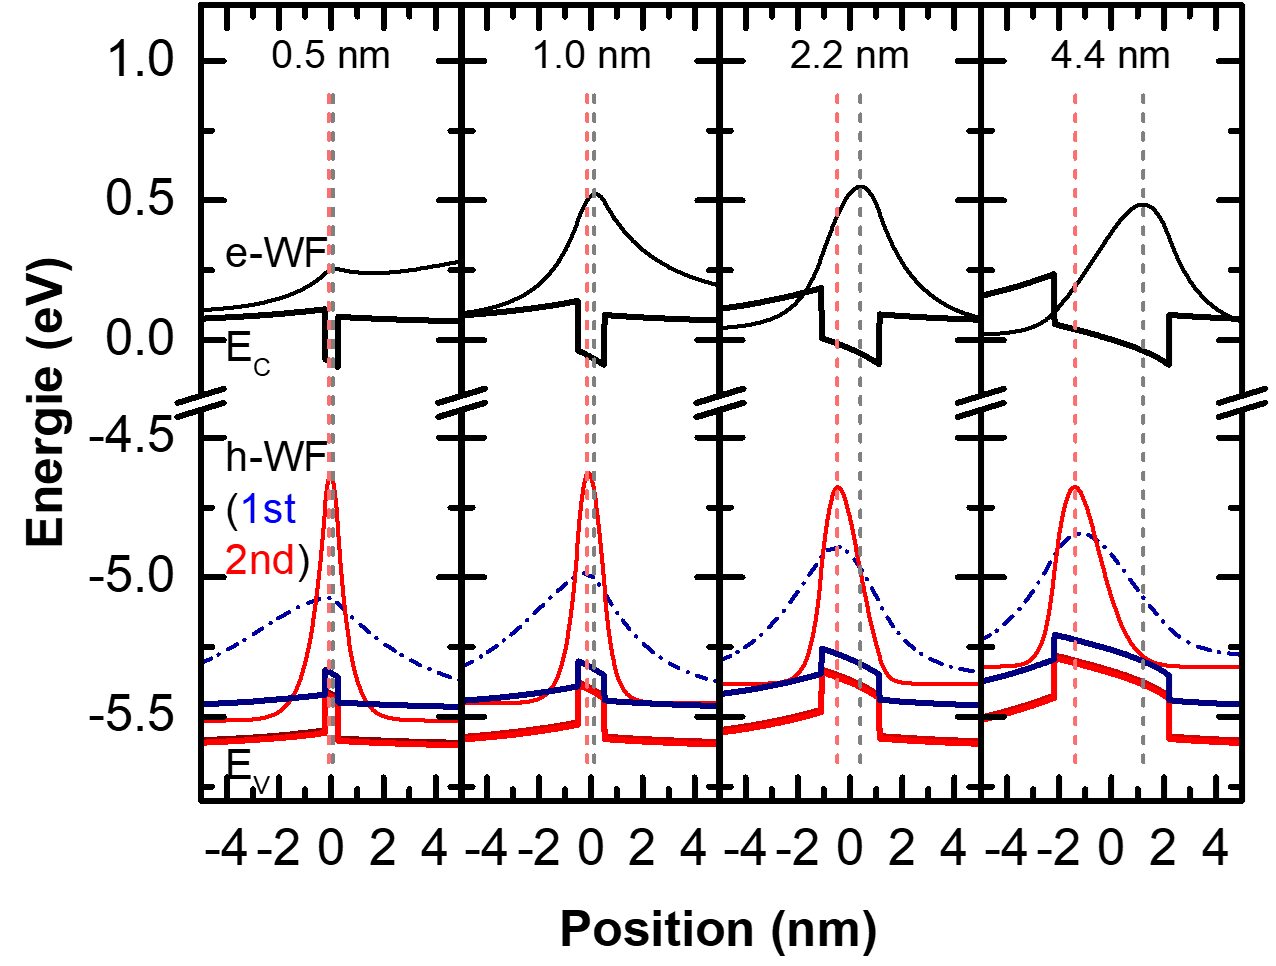
\includegraphics[width=\textwidth]{Bilder/MQWdickenSerie/Simu1.png}
		\caption{Simulation der Elektron- und Lochwellenfunktion im Bändermodell mit QW in einem Bereich von $-4$ bis $4 \thinspace nm$ für verschiedene Dicken. Simulation von Christoph Reich.}
    \label{fig:simu1}
  \end{minipage}
	\hfill
  \begin{minipage}[t]{0.49\textwidth}
    \centering
    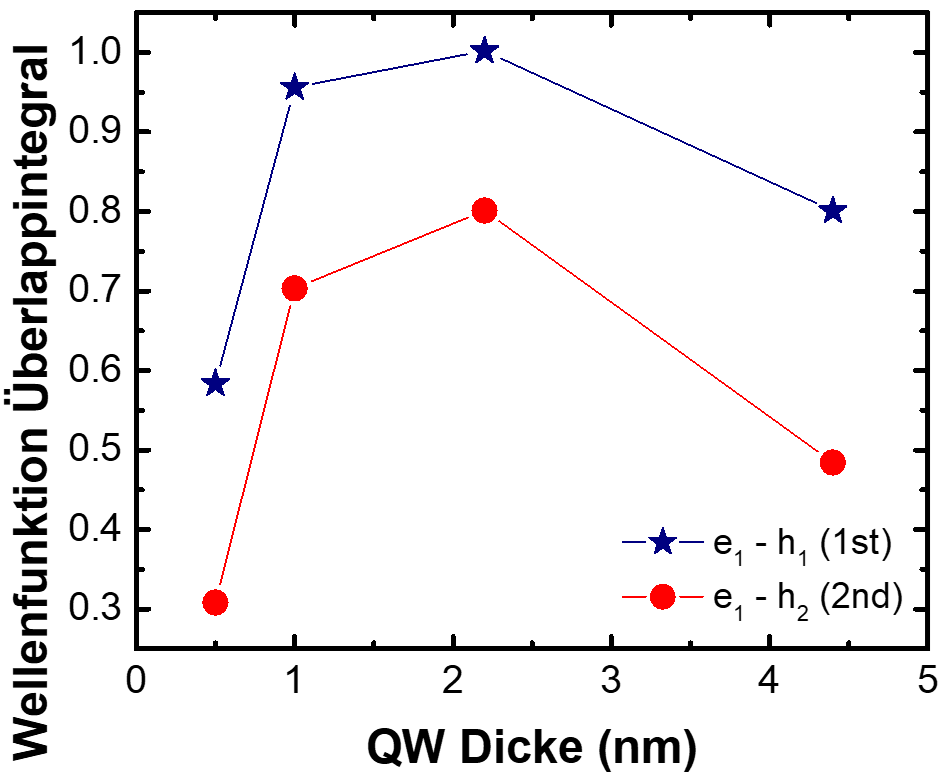
\includegraphics[width=\linewidth]{Bilder/MQWdickenSerie/Simu2.png}
		\caption{Wellenfunktion Überlappintegral in Abhängigkeit der QW-Dicke. Simulation von Christoph Reich.}
    \label{fig:simu2}
  \end{minipage}
\end{figure}
\noindent 
Abbildung \ref{fig:simu1} und \ref{fig:simu2} zeigen Modellberechnungen von Christoph Reich basierend auf der \textbf{k$\cdot$p}-Theorie für variierende QW-Dicken. In Abbildung \ref{fig:simu1} sind die Elektron und Lochwellenfunktion im Bändermodell für die vier verschiedenen Dicken von 
$d=0.5,1.0,2.2,4 \thinspace nm$ dargestellt. 
\newline
Dazu passend zeigt Abbildung \ref{fig:simu2} die zugehörigen Überlappintegrale der Wellenfunktionen.
Das Überlappintegral ist ein Maß für die strahlende Rekombination und je höher der Wert, umso größer ist deren Anteil an der effektiven Rekombinationsrate (Gl. \ref{eq:iqe2}). 
\newline
Somit ist für QW-Dicken von $1.0 \thinspace nm- 2.0 \thinspace nm$ der höchste B-Parameter, der sich aus dem Produkt von Überlappintegral und B-Parameter des Materials zusammensetzt, für die strahlende Rekombination zu erwarten. Bei Annahme, dass Auger-Rekombination und nicht-strahlende Rekombination gleich bleiben, werden auch die höchsten IQEs erwartet. Somit bestätigen die Simulationen die experimentellen Ergebnisse.
\newline
Des Weiteren zeigen die Simulation, dass für eine QW-Dicke von $0,5 \thinspace nm$ die IQE im Vergleich geringer ausfällt, da das Überlappintegral durch den geringeren Ladungsträgereinschluss am kleinsten ausfällt. 

\section{Zusammenfassung}

Die Ergebnisse dieses Kapitels zeigen, dass die QW-Dicke einen eindeutigen Einfluss auf die Rekombination und damit auf die IQE hat. Es wurde experimentell gezeigt und durch \textbf{k$\cdot$p}-Simulationen bestätigt, dass QW-Dicken von $1.0 \thinspace nm- 2.2 \thinspace nm$ die höchsten IQEs und somit das beste Verhältnis zwischen Ladungsträgereinschluss und Screening liefern.
\newline
Die gemessenen IQEs für die Proben mit dotierten und undotierten Barrieren liegen zwischen $0.121$ und $0.145$ und sind somit vergleichbar. Es zeigte sich, dass eine Dotierung in den Barrieren im Bereich geringer Anregungsleistungsdichten zu höheren IQEs führt, diese in Abhängigkeit der Anregungsleistungsdichte jedoch im Vergleich weniger stark ansteigen.
\newline
Weiter wurde gezeigt, dass die Emissionsenergien der undotierten Proben durch das Screening des QCSE mit zunehmender Ladungsträgerdichte steigen und für die Serie mit dotierten Barrieren aufgrund der größeren Anzahl an Ladungsträgern, die den QCSE reduzieren, konstant bleiben.
